\documentclass{article}

\usepackage{amsmath, amssymb}
\usepackage{tikz}
\usepackage{graphicx}
\usepackage{caption}
\usepackage[margin=1in, landscape]{geometry}
\usetikzlibrary{shapes, arrows, positioning, fit, calc}
\usetikzlibrary{shapes.geometric, arrows.meta, positioning, calc, decorations.pathreplacing}

% Page numbering
\usepackage{fancyhdr}
\pagestyle{fancy}
\fancyhf{}
\fancyfoot[C]{\thepage}
\renewcommand{\headrulewidth}{0pt}

\begin{document}

% Title Page
\begin{center}
    \vspace*{3cm}
    {\Huge\bfseries Transformer Architecture\\[0.5cm]
    Implementation Details}\\[2cm]
    {\Large Forward \& Backward Pass Analysis}\\[1cm]
    {\large with Tensor Parallelism}\\[3cm]
    \today
\end{center}

\clearpage

% Table of Contents
\tableofcontents

\clearpage

% ============================================================
% CHAPTER 1: SINGLE NODE TRANSFORMER
% ============================================================
\section{Single Node Transformer}

This chapter covers the complete forward and backward pass of a Transformer model running on a single node (no parallelism).

\clearpage

% ---- 1.1 Overview ----
\subsection{Overall Architecture \& Data Flow}

The following diagram shows the high-level architecture of a Transformer layer, including both forward and backward passes.

\vspace{1cm}

\resizebox{\linewidth}{!}{%
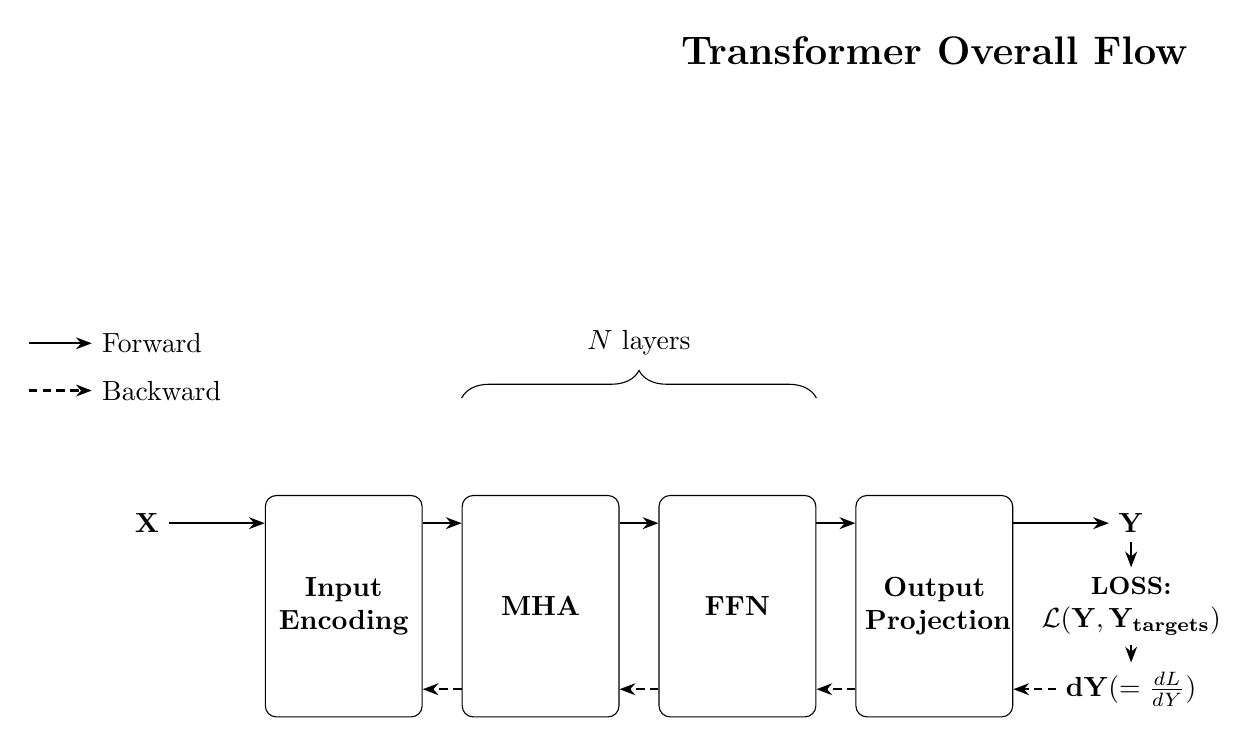
\begin{tikzpicture}[
    node distance=2.5cm,
    >=stealth,
    block/.style={rectangle, draw=black, fill=white, text width=5em, text centered, rounded corners, minimum height=8em, font=\bfseries},
    forward/.style={-{Stealth[length=2mm]}, thick, black},
    backward/.style={-{Stealth[length=2mm]}, thick, black, densely dashed},
    io/.style={text centered, font=\bfseries}
]
    % Title
    \node[font=\Large\bfseries] at (10, 6) {Transformer Overall Flow};

    % Forward path nodes (horizontal)
    \node (input) [io] {$\mathbf{X}$};
    \node (encoding) [block, right of=input, yshift=-3em] {Input\\Encoding};
    \node (mha) [block, right of=encoding] {MHA};
    \node (mlp) [block, right of=mha] {FFN};
    \node (output) [block, right of=mlp] {Output\\Projection};
    \node (pred) [io, right of=output, yshift=3em] {$\mathbf{Y}$};
    \node (loss) [align=center, io, right of=output] {\small LOSS:\\$\mathcal{L}(\mathbf{Y,Y_\text{targets}})$};
    \node (gradient) [io, right of=output, yshift=-3em] {$\mathbf{dY}(=\frac{dL}{dY})$};

    % Forward arrows (upper part of blocks)
    \draw [forward] (input) -- ([yshift=3em]encoding.west);
    \draw [forward] ([yshift=3em]encoding.east) -- ([yshift=3em]mha.west);
    \draw [forward] ([yshift=3em]mha.east) -- ([yshift=3em]mlp.west);
    \draw [forward] ([yshift=3em]mlp.east) -- ([yshift=3em]output.west);
    \draw [forward] ([yshift=3em]output.east) -- (pred);
    \draw [forward] (pred) -- (loss);
    \draw [backward] (loss) -- (gradient);

    % Backward arrows (lower part of blocks)
    \draw [backward] (gradient) -- ([yshift=-3em]output.east);
    \draw [backward] ([yshift=-3em]output.west) -- ([yshift=-3em]mlp.east);
    \draw [backward] ([yshift=-3em]mlp.west) -- ([yshift=-3em]mha.east);
    \draw [backward] ([yshift=-3em]mha.west) -- ([yshift=-3em]encoding.east);

    % Brace for layer repetition
    \draw[decorate, decoration={brace, amplitude=10pt}]
        ([yshift=3.5em]mha.north west) -- ([yshift=3.5em]mlp.north east)
        node[midway, above=12pt, font=\normalsize] {$N$ layers};

    % Labels (Legend)
    \coordinate (legend) at ([xshift=-1.5cm, yshift=6.5em]input);
    \draw[forward] (legend) -- ++(0.8,0) node[right, font=\normalsize] {Forward};
    \draw[backward] ([yshift=-0.6cm]legend) -- ++(0.8,0) node[right, font=\normalsize] {Backward};

\end{tikzpicture}%
}

\clearpage

% ---- 1.2 Input Embedding ----
\subsection{Input Embedding Layer}

The input embedding layer converts token indices into dense vector representations and adds positional encodings.

\vspace{1cm}

\subsubsection{Forward Pass}
\documentclass{article}

\usepackage{amsmath, amssymb}
\usepackage{tikz}
\usepackage{graphicx}
\usepackage{caption}
\usepackage[margin=1in, landscape]{geometry}
\usetikzlibrary{shapes, arrows, positioning, fit, calc}

\begin{document}

% ---------- Input Embedding -> (to MHA) ----------
\noindent
\resizebox{\linewidth}{!}{%
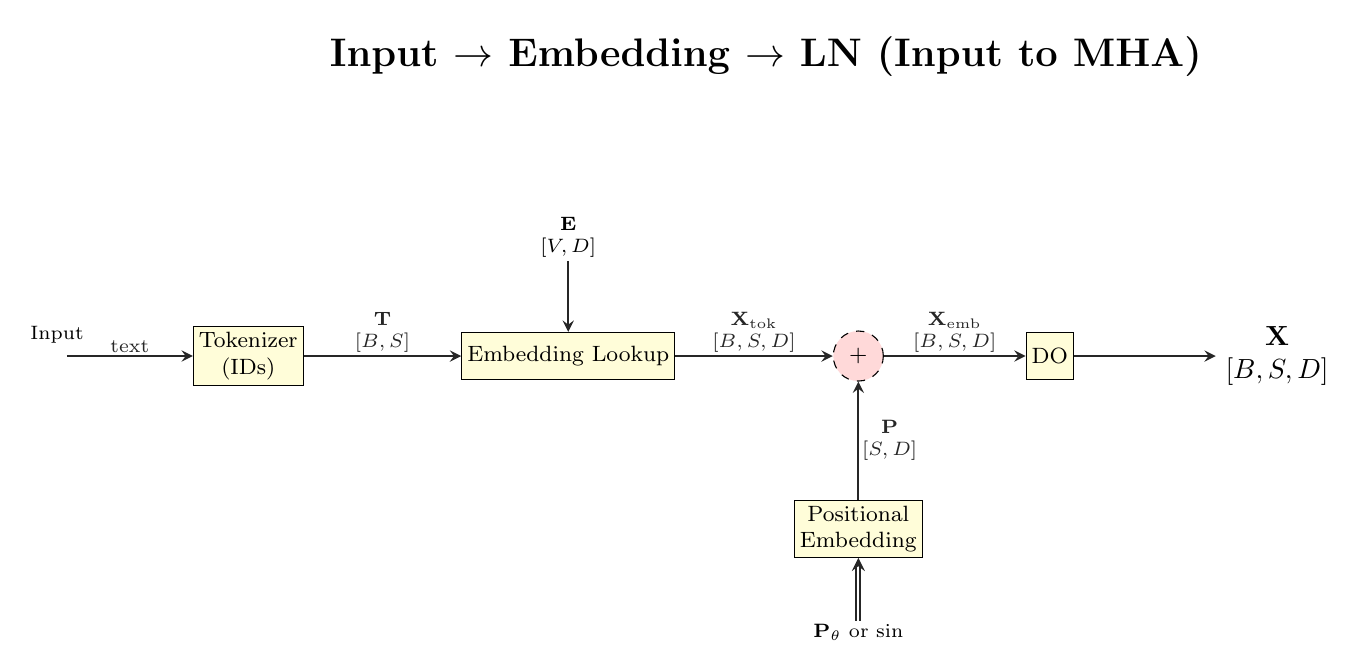
\begin{tikzpicture}[
  >=stealth,
  auxnode/.style={draw, rectangle, fill=yellow!15, minimum height=6mm, inner sep=2pt, font=\footnotesize, align=center},
  mulnode/.style={draw, circle, fill=green!15, minimum size=6mm, font=\footnotesize, align=center},
  addnode/.style={draw, circle, dashed, fill=red!15, minimum size=6mm, font=\footnotesize, align=center},
  flow/.style={->, thick, black!85},
  flow2/.style={->, double, thick, black!85},
  dimlabel/.style={font=\scriptsize, inner sep=1pt, align=center}
]

\node[font=\Large\bfseries] at (9, 3.8) {Input $\rightarrow$ Embedding $\rightarrow$ LN (Input to MHA)};

% nodes
\node (RawText) at (0,0) {};
\node[auxnode, align=center] (Tok)   [right=1.6cm of RawText] {Tokenizer\\(IDs)};
\node[auxnode, align=center] (Lookup)[right=2.0cm of Tok]     {Embedding Lookup};
\node[addnode, minimum size=6mm] (Sum) [right=2.0cm of Lookup] {+};
\node[auxnode, align=center] (PosE)  [below=1.5cm of Sum]  {Positional\\Embedding};
\node[auxnode] (Drop) [right=1.8cm of Sum] {DO};
\node (OUTPUT)   [align=center, right=1.8cm of Drop]   {$\mathbf{X}$\\$[B,S,D]$};

% parameter/const “double” edges
\node[dimlabel] (Eparam) [align=center, above=0.9cm of Lookup] {$\mathbf{E}$\\$[V,D]$};
\node[dimlabel] (Pparam) [align=center, below=0.8cm of PosE]   {$\mathbf{P}_{\theta}$ or sin};

% flows
\draw[flow] (RawText) -- (Tok) node[dimlabel, midway, above]
  {$\text{text}$};
\draw[flow] (Tok) -- (Lookup) node[dimlabel, midway, above]
  {$\mathbf{T}$\\$[B,S]$};

% Embedding matrix E
\draw[flow] (Eparam) -- (Lookup);

% Lookup -> Sum (token embeddings)
\draw[flow] (Lookup) -- (Sum) node[dimlabel, midway, above]
  {$\mathbf{X}_{\text{tok}}$\\$[B,S,D]$};

% Positional embedding path
\draw[flow] (PosE) -- (Sum) node[dimlabel, midway, right]
  {$\mathbf{P}$\\$[S,D]$};

% Optional: show P as parameter (sinusoidal/learned)
\draw[flow2] (Pparam) -- (PosE) ;

\draw[flow] (Sum) -- (Drop) node[dimlabel, midway, above]
  {$\mathbf{X}_{\text{emb}}$\\$[B,S,D]$};
\draw[flow] (Drop) -- (OUTPUT);

% labels for start and destination
\node[dimlabel, above=0.0cm of RawText] {Input};

\end{tikzpicture}%
}

\newpage
\renewcommand{\arraystretch}{1.2}
\small

% -------- Operations (Ops) --------
\begin{center}
\textbf{Operations (Ops)}
\begin{tabular}{llll}
\hline
\textbf{Abbrev} & \textbf{Name} & \textbf{Type / Shape} & \textbf{Notes} \\
\hline
Tokenizer & Tokenizer (IDs) & op & Maps raw text $\to$ integer ids $\mathbf{T}\in\mathbb{Z}^{[B,S]}$. \\
Embedding Lookup & Embedding Lookup & op & Gathers rows from $\mathbf{E}\in\mathbb{R}^{V\times D}$ using ids $\mathbf{T}$. \\
$+$ & Element-wise Add (dashed circle) & op & Adds token and positional embeddings; broadcasting over $B,S$ if needed. \\
DO & Dropout & op & Training-time stochastic dropout on $\mathbf{X}_{\text{emb}}$; identity at inference. \\
\textit{(none)} & Broadcast $\mathrm{BC}_{B,S}(\cdot)$ & op & Expands $[S,D]$ (or $[D]$) to $[B,S,D]$ across batch/sequence. \\
\hline
\end{tabular}
\end{center}

\vspace{0.8em}

% -------- Data Tensors (Values) --------
\begin{center}
\textbf{Data Tensors (Values)}
\begin{tabular}{llll}
\hline
\textbf{Symbol} & \textbf{Name} & \textbf{Shape} & \textbf{Notes} \\
\hline
text & Raw input text & — & Character/byte stream before tokenization. \\
$\mathbf{T}$ & Token ids & $[B,S]$ & Output of Tokenizer; integers in $\{0,\dots,V{-}1\}$. \\
$\mathbf{E}$ & Embedding matrix (params) & $[V,D]$ & Trainable; each vocab entry has a $D$-dim vector. \\
$\mathbf{X}_{\text{tok}}$ & Token embeddings & $[B,S,D]$ & $\mathrm{lookup}(\mathbf{E}, \mathbf{T})$. \\
$\mathbf{P}$ & Positional embedding & $[S,D]$ (or $[B,S,D]$) & Learned $\mathbf{P}_\theta$ \textbf{or} sinusoidal (fixed); broadcast to $[B,S,D]$. \\
$\mathbf{X}_{\text{emb}}$ & Sum of token+pos & $[B,S,D]$ & $\mathbf{X}_{\text{tok}} + \mathrm{BC}_{B,S}(\mathbf{P})$. \\
$\mathbf{X}$ & Input to MHA & $[B,S,D]$ & After dropout (DO); goes to LN/MHA stack. \\
$\mathbf{P}_\theta$ & Learned pos. params & matches $\mathbf{P}$ & Used when positions are trainable; otherwise “sin” denotes fixed sinusoidal. \\
\hline
\multicolumn{4}{l}{\textbf{Shape symbols:}\; $B$=batch size,\; $S$=sequence length,\; $D$=model dim,\; $V$=vocab size.} \\
\multicolumn{4}{l}{\textbf{Notes:}\; In practice, $\mathbf{P}$ may be pre-broadcast to $[B,S,D]$ or added per-token with implicit broadcasting.} \\
\hline
\end{tabular}
\end{center}

\end{document}


\clearpage

\subsubsection{Operations Summary}
\renewcommand{\arraystretch}{1.2}
\small

\begin{center}
\textbf{Operations (Ops)}
\begin{tabular}{llll}
\hline
\textbf{Abbrev} & \textbf{Name} & \textbf{Type / Shape} & \textbf{Notes} \\
\hline
Tokenizer & Tokenizer (IDs) & op & Maps raw text $\to$ integer ids $\mathbf{T}\in\mathbb{Z}^{[B,S]}$. \\
Embedding Lookup & Embedding Lookup & op & Gathers rows from $\mathbf{E}\in\mathbb{R}^{V\times D}$ using ids $\mathbf{T}$. \\
$+$ & Element-wise Add (dashed circle) & op & Adds token and positional embeddings; broadcasting over $B,S$ if needed. \\
DO & Dropout & op & Training-time stochastic dropout on $\mathbf{X}_{\text{emb}}$; identity at inference. \\
\textit{(none)} & Broadcast $\mathrm{BC}_{B,S}(\cdot)$ & op & Expands $[S,D]$ (or $[D]$) to $[B,S,D]$ across batch/sequence. \\
\hline
\end{tabular}
\end{center}

\vspace{0.8em}

\begin{center}
\textbf{Data Tensors (Values)}
\begin{tabular}{llll}
\hline
\textbf{Symbol} & \textbf{Name} & \textbf{Shape} & \textbf{Notes} \\
\hline
text & Raw input text & — & Character/byte stream before tokenization. \\
$\mathbf{T}$ & Token ids & $[B,S]$ & Output of Tokenizer; integers in $\{0,\dots,V{-}1\}$. \\
$\mathbf{E}$ & Embedding matrix (params) & $[V,D]$ & Trainable; each vocab entry has a $D$-dim vector. \\
$\mathbf{X}_{\text{tok}}$ & Token embeddings & $[B,S,D]$ & $\mathrm{lookup}(\mathbf{E}, \mathbf{T})$. \\
$\mathbf{P}$ & Positional embedding & $[S,D]$ (or $[B,S,D]$) & Learned $\mathbf{P}_\theta$ \textbf{or} sinusoidal (fixed); broadcast to $[B,S,D]$. \\
$\mathbf{X}_{\text{emb}}$ & Sum of token+pos & $[B,S,D]$ & $\mathbf{X}_{\text{tok}} + \mathrm{BC}_{B,S}(\mathbf{P})$. \\
$\mathbf{X}$ & Input to MHA & $[B,S,D]$ & After dropout (DO); goes to LN/MHA stack. \\
$\mathbf{P}_\theta$ & Learned pos. params & matches $\mathbf{P}$ & Used when positions are trainable; otherwise “sin” denotes fixed sinusoidal. \\
\hline
\multicolumn{4}{l}{\textbf{Shape symbols:}\; $B$=batch size,\; $S$=sequence length,\; $D$=model dim,\; $V$=vocab size.} \\
\multicolumn{4}{l}{\textbf{Notes:}\; In practice, $\mathbf{P}$ may be pre-broadcast to $[B,S,D]$ or added per-token with implicit broadcasting.} \\
\hline
\end{tabular}
\end{center}


\clearpage

% ---- 1.3 Multi-Head Attention ----
\subsection{Multi-Head Attention (MHA)}

Multi-Head Attention enables the model to jointly attend to information from different representation subspaces.

\vspace{1cm}

\subsubsection{Forward Pass}
\resizebox{\linewidth}{!}{%
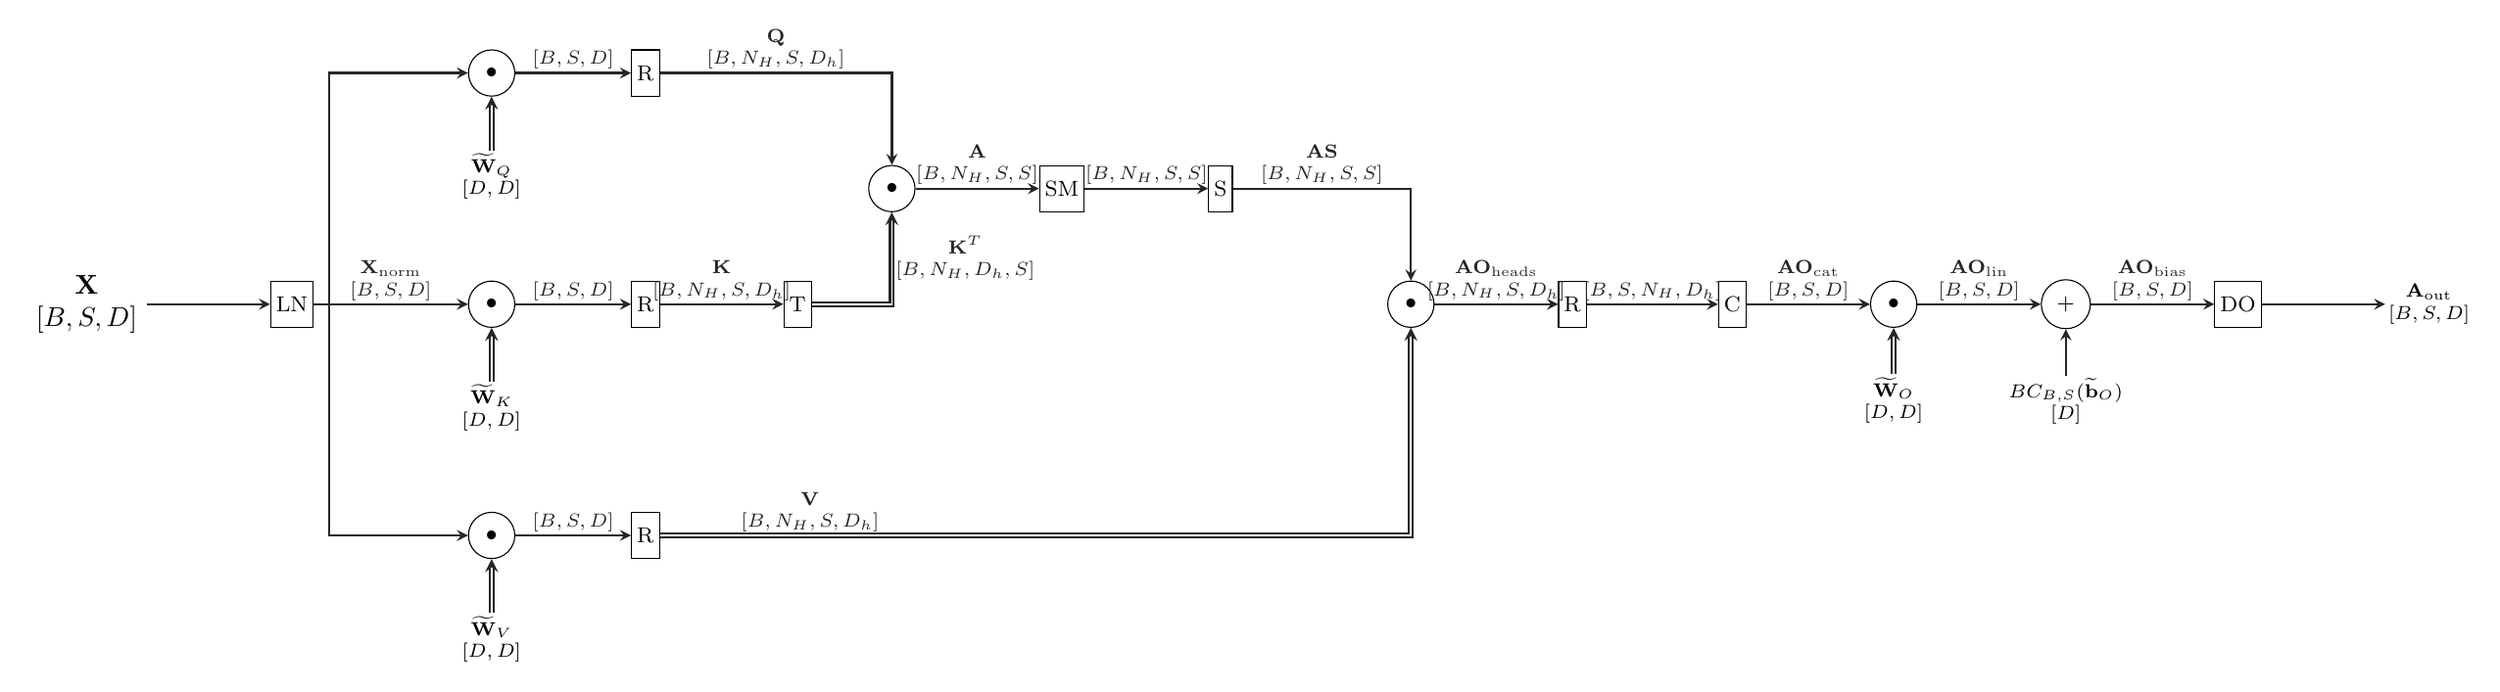
\begin{tikzpicture}[
  every node/.style={transform shape},
  >=stealth,
  auxnode/.style={draw, rectangle, fill=white, minimum height=6mm, inner sep=2pt, font=\footnotesize, align=center},
  mulnode/.style={draw, circle, fill=white, minimum size=6mm, font=\footnotesize, align=center},
  addnode/.style={draw, circle, fill=white, minimum size=6mm, font=\footnotesize, align=center},
  flow/.style={->, thick, black!85},
  flow2/.style={->, double, thick, black!85},
  dimlabel/.style={font=\scriptsize, inner sep=1pt, align=center}
]
% \node[font=\Large\bfseries] at (8, 4.5) {Multi-Head Attention Forward Pass};

\node (Input) at (0.5, 0) [align=center] {$\mathbf{X}$\\$[B,S,D]$};
\node[auxnode] (LN) [right=1.6cm of Input] {LN};

\node[mulnode] (Proj_Q) [right=2.0cm of LN, yshift=3.0cm] {$\bullet$};
\node[auxnode] (R_Q) [right=1.5cm of Proj_Q] {R};

\node[mulnode] (Proj_K) [right=2.0cm of LN, yshift=0cm] {$\bullet$};
\node[auxnode] (R_K) [right=1.5cm of Proj_K] {R};

\node[mulnode] (Proj_V) [right=2.0cm of LN, yshift=-3.0cm] {$\bullet$};
\node[auxnode] (R_V) [right=1.5cm of Proj_V] {R};

\node[dimlabel] (WQ) [align=center, below=0.7cm of Proj_Q] {$\widetilde{\mathbf{W}}_{Q}$\\$[D,D]$};
\node[dimlabel] (WK) [align=center, below=0.7cm of Proj_K] {$\widetilde{\mathbf{W}}_{K}$\\$[D,D]$};
\node[dimlabel] (WV) [align=center, below=0.7cm of Proj_V] {$\widetilde{\mathbf{W}}_{V}$\\$[D,D]$};

\node[auxnode] (T_K) [right=1.6cm of R_K] {T};
\node[mulnode] (QK) [right=2.7cm of R_Q, yshift=-1.5cm] {$\bullet$};
\node[auxnode] (SM) [right=1.6cm of QK] {SM};
\node[auxnode] (Soft) [right=1.6cm of SM] {S};
\node[mulnode] (PV) [right=2.0cm of Soft, yshift=-1.5cm] {$\bullet$};

\node[auxnode] (R_Merge) [right=1.6cm of PV] {R};
\node[auxnode] (Cat) [right=1.7cm of R_Merge] {C};

\node[mulnode] (OProj) [right=1.6cm of Cat] {$\bullet$};
\node[dimlabel] (WO_FWD) [align=center, below=0.6cm of OProj] {$\widetilde{\mathbf{W}}_{O}$\\$[D,D]$};
\node[addnode] (AddB) [right=1.6cm of OProj] {+};
\node[dimlabel] (BO) [align=center, below=0.6cm of AddB] {$BC_{B,S}(\widetilde{\mathbf{b}}_{O})$\\$[D]$};
\node[auxnode] (Drop) [right=1.6cm of AddB] {DO};
\node[dimlabel] (Aout) [align=center, right=1.6cm of Drop] {$\mathbf{A}_{\text{out}}$\\$[B,S,D]$};

\draw[flow] (Input) -- (LN);

\draw[flow] (LN.east) -- ++(0.2,0) |- (Proj_Q.west);
\draw[flow] (LN) -- (Proj_K.west) node[dimlabel, midway, above]{$\mathbf{X}_{\text{norm}}$\\$[B,S,D]$};
\draw[flow] (LN.east) -- ++(0.2,0) |- (Proj_V.west);

\draw[flow2] (WQ) -- (Proj_Q);
\draw[flow2] (WK) -- (Proj_K);
\draw[flow2] (WV) -- (Proj_V);

\draw[flow] (Proj_Q) -- (R_Q) node[dimlabel, midway, above]{$[B,S,D]$};
\draw[flow] (Proj_K) -- (R_K) node[dimlabel, midway, above]{$[B,S,D]$};
\draw[flow] (Proj_V) -- (R_V) node[dimlabel, midway, above]{$[B,S,D]$};

\draw[flow] (R_Q) -| (QK) node[dimlabel, near start, above]{$\mathbf{Q}$\\$[B,N_H,S,D_h]$};
\draw[flow] (R_K) -- (T_K) node[dimlabel, midway, above]{$\mathbf{K}$\\$[B,N_H,S,D_h]$};
\draw[flow2] (T_K) -| (QK) node[dimlabel, near end, right]{$\mathbf{K}^{T}$\\$[B,N_H,D_h,S]$};

\draw[flow] (QK) -- (SM) node[dimlabel, midway, above]{$\mathbf{A}$\\$[B,N_H,S,S]$};
\draw[flow] (SM) -- (Soft) node[dimlabel, midway, above]{$[B,N_H,S,S]$};
\draw[flow] (Soft) -| (PV) node[dimlabel, near start, above]{$\mathbf{AS}$\\$[B,N_H,S,S]$};
\draw[flow2] (R_V) -| (PV) node[dimlabel, pos=0.1, above]{$\mathbf{V}$\\$[B,N_H,S,D_h]$};

\draw[flow] (PV) -- (R_Merge) node[dimlabel, midway, above]{$\mathbf{AO}_{\text{heads}}$\\$[B,N_H,S,D_h]$};
\draw[flow] (R_Merge) -- (Cat) node[dimlabel, midway, above]{$[B,S,N_H,D_h]$};
\draw[flow] (Cat) -- (OProj) node[dimlabel, midway, above]{$\mathbf{AO}_{\text{cat}}$\\$[B,S,D]$};
\draw[flow2] (WO_FWD) -- (OProj);
\draw[flow] (OProj) -- (AddB) node[dimlabel, midway, above]{$\mathbf{AO}_{\text{lin}}$\\$[B,S,D]$};
\draw[flow] (BO) -- (AddB);
\draw[flow] (AddB) -- (Drop) node[dimlabel, midway, above]{$\mathbf{AO}_{\text{bias}}$\\$[B,S,D]$};
\draw[flow] (Drop) -- (Aout);
\end{tikzpicture}%
}


\clearpage

\subsubsection{Backward Pass}
\resizebox{\linewidth}{!}{%
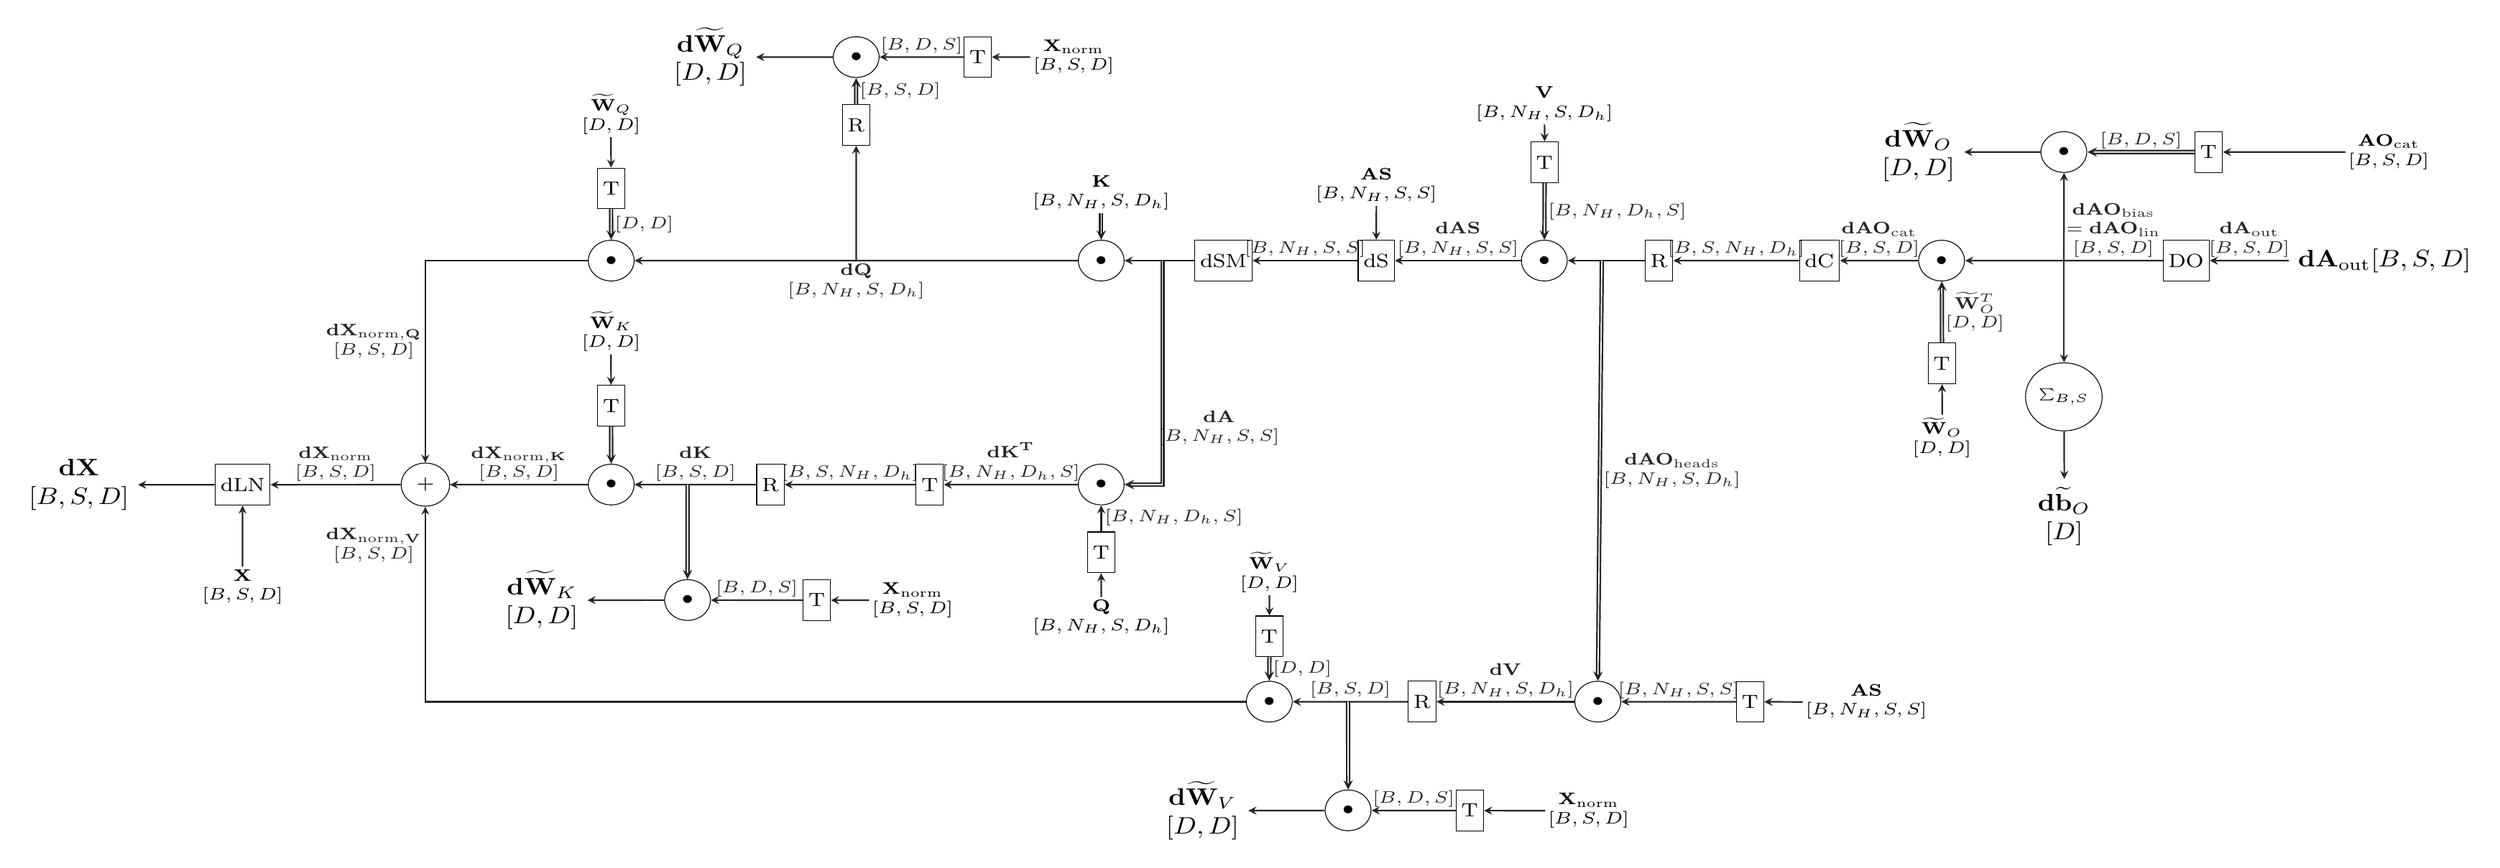
\begin{tikzpicture}[
  every node/.style={transform shape},
  >=stealth,
  auxnode/.style={draw, rectangle, fill=white, minimum height=6mm, inner sep=2pt, font=\footnotesize, align=center},
  mulnode/.style={draw, circle, fill=white, minimum size=6mm, font=\footnotesize, align=center},
  addnode/.style={draw, circle, fill=white, minimum size=6mm, font=\footnotesize, align=center},
  sumnode/.style={draw, circle, fill=white, minimum size=6mm, font=\tiny, align=center},
  flow/.style={->, thick, black!85},
  flow2/.style={->, double, thick, black!85},
  dimlabel/.style={font=\scriptsize, inner sep=1pt, align=center},
  gradflow/.style={->, thick, black!85},
  gradweight/.style={->, thick, black!85}
]

\begin{scope}[xscale=1.35, yscale=1.2]

\def\yoffset{-1.0}
\def\dVXyoffset{-6.5}

\coordinate (Grad_Aout_B) at (17.5, \yoffset);
\coordinate (dDrop_center) at (15.9, \yoffset);
\coordinate (ProjGradSplit) at (14.3, \yoffset);
\coordinate (dOProj_center) at (12.7, \yoffset);
\coordinate (C_center) at (11.1, \yoffset);
\coordinate (R_center) at (9.0, \yoffset);
\coordinate (dPV_AS_calc_center) at (7.5, \yoffset);
\coordinate (dSoft_center) at (5.3, \yoffset);
\coordinate (dSM_calc_center) at (3.3, \yoffset);
\coordinate (dV_calc_center) at (8.2, \dVXyoffset+\yoffset);
\coordinate (R_V_bwd_center) at (5.9, \dVXyoffset+\yoffset);
\coordinate (dVX_calc_center) at (3.9, \dVXyoffset+\yoffset);
\coordinate (dQK_calc_Q_center) at (1.7, \yoffset);
\coordinate (dQK_calc_K_center) at (1.7, -3.3+\yoffset);
\coordinate (K_BWD_input_center) at (1.7, 1.0+\yoffset);
\coordinate (T_Q_bwd_center) at (1.7, -4.3+\yoffset);

% \node[font=\Large\bfseries] at (8, 4.6+\yoffset) {Multi-Head Attention Backward Pass};

\node (Grad_Aout_B) at (18.5, \yoffset) {$\mathbf{dA}_{\text{out}}$\\$[B,S,D]$};
\node[auxnode] (DO) at (dDrop_center) {DO};
\node[mulnode] (dOProj) at (dOProj_center) {$\bullet$};

\node[auxnode] (T_WO) [below=0.9cm of dOProj] {T};
\node[dimlabel] (WO_BWD) [below=0.45cm of T_WO] {$\widetilde{\mathbf{W}}_{O}$\\$[D,D]$};

\node[mulnode] (dWO_calc) at ($(ProjGradSplit)+(0, 1.6)$) {$\bullet$};
\node[align=center, left=1.0cm of dWO_calc]
  (dWO_GRAD) {$\mathbf{d}\widetilde{\mathbf{W}}_{O}$\\$[D,D]$};
\node[auxnode] (T_AO_in) [right=1.4cm of dWO_calc] {T};
\node[dimlabel] (AO_in_local_label) [right=1.6cm of T_AO_in] {$\mathbf{AO}_{\text{cat}}$\\$[B,S,D]$};

\node[auxnode] (C) at (C_center) {dC};
\node[auxnode] (R) at (R_center) {R};

\node[mulnode] (dPV_AS_calc) at (dPV_AS_calc_center) {$\bullet$};
\node[auxnode] (dSoft) at (dSoft_center) {dS};
\node[auxnode] (dSM_calc) at (dSM_calc_center) {dSM};

\node[mulnode] (dQK_calc_Q) at (dQK_calc_Q_center) {$\bullet$};
\node[mulnode] (dQX_proj_calc) [left=5.8cm of dQK_calc_Q] {$\bullet$};

\node[mulnode] (dQK_calc_K) at (dQK_calc_K_center) {$\bullet$};
\node[mulnode] (dKX_proj_calc) [left=5.8cm of dQK_calc_K] {$\bullet$};

\node[dimlabel] (K_BWD_input) at (K_BWD_input_center) {$\mathbf{K}$\\$[B,N_H,S,D_h]$};
\node[auxnode] (T_Q_bwd) at (T_Q_bwd_center) {T};
\node[dimlabel] (Q_BWD_input) [below=0.35cm of T_Q_bwd] {$\mathbf{Q}$\\$[B,N_H,S,D_h]$};

\node[dimlabel] (V_FWD) [above=1.7cm of dPV_AS_calc] {$\mathbf{V}$\\$[B,N_H,S,D_h]$};
\node[auxnode] (T_V_bwd) [below=0.25cm of V_FWD] {T};

\node[mulnode] (dV_calc) at (dV_calc_center) {$\bullet$};
\node[auxnode] (T_AS_bwd) [right=1.5cm of dV_calc] {T};
\node[dimlabel] (AS_BWD_for_V) [right=0.5cm of T_AS_bwd] {$\mathbf{AS}$\\$[B,N_H,S,S]$};

\node[auxnode] (R_V_bwd) at (R_V_bwd_center) {R};
\node[mulnode] (dVX_calc) at (dVX_calc_center) {$\bullet$};

\node[auxnode] (T_WV) [above=0.35cm of dVX_calc] {T};
\node[dimlabel] (WV_BWD) [above=0.3cm of T_WV] {$\widetilde{\mathbf{W}}_{V}$\\$[D,D]$};

\node[sumnode] (Sum_dBO) [below=1.5cm of ProjGradSplit] {$\sum_{B, S}$};
\node (dBO) [align=center, below=0.7cm of Sum_dBO] {$\mathbf{d}\widetilde{\mathbf{b}}_{O}$\\$[D]$};

\draw[gradflow] (Grad_Aout_B) -- (DO)
  node[dimlabel, midway, above]{$\mathbf{dA}_{\text{out}}$\\$[B,S,D]$};

\draw[gradflow] (DO) -- (dOProj)
  node[dimlabel, pos=0.25, above]{$\mathbf{dAO}_{\text{bias}}$\\$=\mathbf{dAO}_{\text{lin}}$\\$[B,S,D]$};

\draw[gradflow] (ProjGradSplit) -- (dWO_calc.south);
\draw[gradflow] (ProjGradSplit) -- ([yshift=-0.75cm]ProjGradSplit) -| (Sum_dBO.north);

\draw[gradflow] (dOProj) -- (C)
  node[dimlabel, midway, above]{$\mathbf{dAO}_{\text{cat}}$\\$[B,S,D]$};
\draw[gradflow] (C) -- (R)
  node[dimlabel, midway, above]{$[B,S,N_H,D_h]$};

\coordinate (R_split_point) at ($(dPV_AS_calc)!0.5!(R)$);
\draw[gradflow] (R.west) -- (dPV_AS_calc.east);
\draw[flow2] (R_split_point) -- (dV_calc.north)
  node[dimlabel, midway, right]{$\mathbf{dAO}_{\text{heads}}$\\$[B,N_H,S,D_h]$};

\draw[gradflow] (V_FWD.south) -- (T_V_bwd.north);
\draw[flow2] (T_V_bwd.south) -- (dPV_AS_calc.north)
  node[dimlabel, midway, right]{$[B,N_H,D_h,S]$};
\draw[gradflow] (dPV_AS_calc.west) -- (dSoft.east)
  node[dimlabel, midway, above]{$\mathbf{dAS}$\\$[B,N_H,S,S]$};

\node (AS_BWD_dS) [dimlabel, above=0.5cm of dSoft] {$\mathbf{AS}$\\$[B,N_H,S,S]$};
\draw[gradflow] (AS_BWD_dS.south) -- (dSoft.north);
\draw[gradflow] (dSoft.west) -- (dSM_calc.east)
  node[dimlabel, midway, above]{$[B,N_H,S,S]$};

\coordinate (dA_Split_X) at ($(dSM_calc_center)!0.5!(dQK_calc_Q_center)$);
\coordinate (dA_Split) at (dA_Split_X |- dQK_calc_Q.east);
\draw[gradflow] (dSM_calc.west) -- (dQK_calc_Q.east);
\draw[flow2] (dA_Split) -- (dA_Split |- dQK_calc_K.east) -- (dQK_calc_K.east)
  node[dimlabel, pos=-1.5, above, yshift=15]{$\mathbf{dA}$\\$[B,N_H,S,S]$};

\draw[flow2] (K_BWD_input.south) -- (dQK_calc_Q.north);
\draw[gradweight] (dQK_calc_Q) -- (dQX_proj_calc)
  node[dimlabel, midway, below]{$\mathbf{dQ}$\\$[B,N_H,S,D_h]$};

\node[auxnode] (T_WQ_bwd) [above=0.45cm of dQX_proj_calc] {T};
\node[dimlabel] (WQ_bwd) [above=0.45cm of T_WQ_bwd] {$\widetilde{\mathbf{W}}_{Q}$\\$[D,D]$};
\draw[flow] (WQ_bwd) -- (T_WQ_bwd);
\draw[flow2] (T_WQ_bwd.south) -- (dQX_proj_calc.north)
  node[dimlabel, midway, right]{$[D,D]$};

\draw[flow] (Q_BWD_input.north) -- (T_Q_bwd.south);
\draw[flow] (T_Q_bwd.north) -- (dQK_calc_K.south)
  node[dimlabel, pos=0.55, right]{$[B,N_H,D_h,S]$};

\node[auxnode] (T_dK) at ($(dQK_calc_K)!0.35!(dKX_proj_calc)$) {T};
\node[auxnode] (R_dK_mid) at ($(T_dK)!0.5!(dKX_proj_calc)$) {R};

\draw[gradweight] (dQK_calc_K) -- (T_dK)
  node[dimlabel, midway, above]{$\mathbf{dK^T}$\\$[B,N_H,D_h,S]$};
\draw[gradweight] (T_dK) -- (R_dK_mid)
  node[dimlabel, midway, above]{$[B,S,N_H,D_h]$};
\draw[gradweight] (R_dK_mid) -- (dKX_proj_calc)
  node[dimlabel, midway, above]{$\mathbf{dK}$\\$[B,S,D]$};

\node[auxnode] (T_WK_bwd) [above=0.55cm of dKX_proj_calc] {T};
\node[dimlabel] (WK_bwd) [above=0.45cm of T_WK_bwd] {$\widetilde{\mathbf{W}}_{K}$\\$[D,D]$};
\draw[gradflow] (WK_bwd) -- (T_WK_bwd);
\draw[flow2] (T_WK_bwd.south) -- (dKX_proj_calc.north);

\draw[gradflow] (AS_BWD_for_V.west) -- (T_AS_bwd.east);
\draw[gradflow] (T_AS_bwd.west) -- (dV_calc.east)
  node[dimlabel, midway, above]{$[B,N_H,S,S]$};
\draw[gradflow] (dV_calc.west) -- (R_V_bwd.east)
  node[dimlabel, midway, above]{$\mathbf{dV}$\\$[B,N_H,S,D_h]$};
\draw[gradflow] (R_V_bwd) -- (dVX_calc.east)
  node[dimlabel, midway, above]{$[B,S,D]$};

\draw[gradflow] (WV_BWD) -- (T_WV);
\draw[flow2] (T_WV) -- (dVX_calc.north)
  node[dimlabel, midway, right]{$[D,D]$};

\node[addnode] (Sum_dXnorm) [left=1.8cm of dKX_proj_calc] {$+$};

\draw[gradweight] (dQX_proj_calc.west) -| node[dimlabel, pos=0.7, left]{$\mathbf{dX}_{\text{norm},\mathbf{Q}}$\\$[B,S,D]$} (Sum_dXnorm.north);
\draw[gradweight] (dKX_proj_calc.west) -- node[dimlabel, midway, above]{$\mathbf{dX}_{\text{norm},\mathbf{K}}$\\$[B,S,D]$} (Sum_dXnorm.east);
\draw[gradweight] (dVX_calc.west) -| node[dimlabel, pos=0.9, left]{$\mathbf{dX}_{\text{norm},\mathbf{V}}$\\$[B,S,D]$} (Sum_dXnorm.south);

\coordinate (dV_branch) at ($(R_V_bwd.west)!0.52!(dVX_calc.east)$);
\node[mulnode] (dWV_mul) at ($(dV_branch)+(0,-1.6cm)$) {$\bullet$};
\draw[flow2] (dV_branch) -- (dWV_mul.north);

\node[auxnode] (T_Xnorm) [right=1.1cm of dWV_mul] {T};
\node[dimlabel] (Xnorm_local) [right=0.8cm of T_Xnorm] {$\mathbf{X}_{\text{norm}}$\\$[B,S,D]$};
\draw[gradflow] (Xnorm_local) -- (T_Xnorm);
\draw[gradflow] (T_Xnorm.west) -- (dWV_mul.east)
  node[dimlabel, midway, above]{$[B,D,S]$};
\node (dWV_out) [align=center, left=1.0cm of dWV_mul] {$\mathbf{d}\widetilde{\mathbf{W}}_{V}$\\$[D,D]$};
\draw[gradweight] (dWV_mul.west) -- (dWV_out);

\coordinate (dQ_branch) at ($(dQK_calc_Q.east)!0.50!(dQX_proj_calc.west)$);
\node[mulnode] (dWQ_mul) at ($(dQ_branch)+(0,3.0cm)$) {$\bullet$};
\node[auxnode] (R_dQ_for_WQ) at ($(dWQ_mul)+(0,-1.0cm)$) {R};
\draw[gradflow]  (dQ_branch) -- (R_dQ_for_WQ.south);
\draw[flow2] (R_dQ_for_WQ.north) -- (dWQ_mul.south)
  node[dimlabel, midway, right]{$[B,S,D]$};

\node[auxnode] (T_XnormQ) [right=1.1cm of dWQ_mul] {T};
\node[dimlabel] (Xnorm_localQ) [right=0.5cm of T_XnormQ] {$\mathbf{X}_{\text{norm}}$\\$[B,S,D]$};
\draw[gradflow] (Xnorm_localQ) -- (T_XnormQ);
\draw[gradflow] (T_XnormQ.west) -- (dWQ_mul.east)
  node[dimlabel, midway, above]{$[B,D,S]$};
\node (dWQ_out) [align=center, left=1.0cm of dWQ_mul] {$\mathbf{d}\widetilde{\mathbf{W}}_{Q}$\\$[D,D]$};
\draw[gradweight] (dWQ_mul.west) -- (dWQ_out);

\coordinate (dK_branch) at ($(R_dK_mid)!0.52!(dKX_proj_calc)$);
\node[mulnode] (dWK_mul) at ($(dK_branch)+(0,-1.7cm)$) {$\bullet$};
\draw[flow2]  (dK_branch) -- (dWK_mul.north);

\node[auxnode] (T_XnormK) [right=1.2cm of dWK_mul] {T};
\node[dimlabel, right=0.5cm of T_XnormK] (Xnorm_localK) {$\mathbf{X}_{\text{norm}}$\\$[B,S,D]$};
\draw[gradflow] (Xnorm_localK) -- (T_XnormK);
\draw[gradflow] (T_XnormK.west) -- (dWK_mul.east)
  node[dimlabel, midway, above]{$[B,D,S]$};
\node (dWK_out) [align=center, left=1.0cm of dWK_mul] {$\mathbf{d}\widetilde{\mathbf{W}}_{K}$\\$[D,D]$};
\draw[gradweight] (dWK_mul.west) -- (dWK_out);

\draw[gradweight] (Sum_dBO) -- (dBO);

\draw[gradflow] (WO_BWD) -- (T_WO);
\draw[flow2] (T_WO) -- (dOProj)
  node[dimlabel, midway, right]{$\widetilde{\mathbf{W}}_{O}^{T}$\\$[D,D]$};
\draw[gradflow] (AO_in_local_label) -- (T_AO_in);
\draw[flow2] (T_AO_in) -- (dWO_calc.east)
  node[dimlabel, midway, above]{$[B,D,S]$};
\draw[gradweight] (dWO_calc) -- (dWO_GRAD);

\node[auxnode] (dLN) [left=1.7cm of Sum_dXnorm] {dLN};
\draw[gradweight] (Sum_dXnorm.west) -- node[dimlabel, midway, above]
  {$\mathbf{dX}_{\text{norm}}$\\$[B,S,D]$} (dLN.east);

\node (dX_OUT) [align=center, left=1.0cm of dLN] {$\mathbf{dX}$\\$[B,S,D]$};
\draw[gradweight] (dLN.west) -- (dX_OUT);

\node[dimlabel] (LNCache) [below=0.9cm of dLN] {$\mathbf{X}$\\$[B,S,D]$};
\draw[gradflow] (LNCache.north) -- (dLN.south);

\end{scope}
\end{tikzpicture}
}


\clearpage

\subsubsection{Operations Summary}
\renewcommand{\arraystretch}{1.2}
\small

\begin{center}
% \textbf{MHA Diagrams: Unified Table (Ops \& Data Tensors)}
\setlength{\tabcolsep}{6pt}
\begin{tabular}{lllll}
\hline
\textbf{Category} & \textbf{Symbol / Abbrev} & \textbf{Name} & \textbf{Shape / Type} & \textbf{Notes} \\
\hline
Ops & LN & Layer Normalization & op & Normalizes per token (last dim $D$). \\
Ops & DO & Dropout & op & Training-time only; identity at inference. \\
Ops & $+$ & Bias Add & op & Adds broadcast bias; see $\mathrm{BC}_{B,S}(\cdot)$. \\
Ops & T & Transpose & op & e.g., $[B,N_H,S,D_h]\!\to\![B,N_H,D_h,S]$. \\
Ops & R & Reshape / Split / Merge & op & $[B,S,D]\!\leftrightarrow\![B,N_H,S,D_h]$. \\
Ops & C & Concatenate & op & $[B,S,N_H,D_h]\!\to\![B,S,D]$. \\
Ops & SM & Scale (+ Mask) & op & Multiply by $1/\sqrt{D_h}$ and apply mask. \\
Ops & S & Softmax & op & Over key length $S$ per head. \\
Ops & $\mathrm{BC}_{B,S}(\cdot)$ & Broadcast & op & Broadcast length-$D$ (or $D_h$) to $[B,S,\cdot]$. \\
Ops & dS & Softmax Backward & op & Backprop through softmax over $S$. \\
Ops & dSM & Scale/Mask Backward & op & Backprop through scaling/masking. \\
Ops & dC & De-concat (Backward) & op & Split grads from concatenated heads. \\
Ops & dLN & LayerNorm Backward & op & Uses cached stats $(\mu,\sigma)$ and $\mathbf{X}$. \\
\hline
Data & $\mathbf{X}$ & Input hidden states & $[B,S,D]$ & Into MHA block (pre-LN). \\
Data & $\mathbf{X}_{\text{norm}}$ & LN output & $[B,S,D]$ & Result of LN($\mathbf{X}$). \\
Data & $\mathbf{Q},\mathbf{K},\mathbf{V}$ & Query/Key/Value & $[B,N_H,S,D_h]$ & From linear projections of $\mathbf{X}_{\text{norm}}$. \\
Data & $\widetilde{\mathbf{W}}_{Q}$ & Q weight & $[D,D]$ & Per-head realized via reshape (drawn fused). \\
Data & $\widetilde{\mathbf{W}}_{K}$ & K weight & $[D,D]$ & Same convention. \\
Data & $\widetilde{\mathbf{W}}_{V}$ & V weight & $[D,D]$ & Same convention. \\
Data & $\widetilde{\mathbf{W}}_{O}$ & Output-proj weight & $[D,D]$ & Maps concatenated heads to model dim. \\
Data & $\widetilde{\mathbf{b}}_{O}$ & Output bias & $[D]$ & Broadcast via $\mathrm{BC}_{B,S}$. \\
Data & $\mathbf{A}$ & Attention scores & $[B,N_H,S,S]$ & $\mathbf{Q}\mathbf{K}^T/\sqrt{D_h}$ (plus mask). \\
Data & $\mathbf{AS}$ & Attention weights & $[B,N_H,S,S]$ & $\mathrm{softmax}(\mathbf{A})$. \\
Data & $\mathbf{AO}_{\text{heads}}$ & Per-head outputs & $[B,N_H,S,D_h]$ & $\mathbf{AS}\cdot\mathbf{V}$. \\
Data & $\mathbf{AO}_{\text{cat}}$ & Concatenated heads & $[B,S,D]$ & After \textit{C}. \\
Data & $\mathbf{AO}_{\text{lin}}$ & Linear output & $[B,S,D]$ & $\mathbf{AO}_{\text{cat}}\widetilde{\mathbf{W}}_{O}$. \\
Data & $\mathbf{AO}_{\text{bias}}$ & Bias-added output & $[B,S,D]$ & $+\;\widetilde{\mathbf{b}}_{O}$. \\
Data & $\mathbf{A}_{\text{out}}$ & MHA output & $[B,S,D]$ & After dropout; to next sublayer. \\
Data & $\mathbf{dA}_{\text{out}}$ & Grad wrt MHA output & $[B,S,D]$ & Backprop signal entering MHA. \\
Data & $\mathbf{dQ},\mathbf{dK},\mathbf{dV}$ & Gradients for Q/K/V & $[B,N_H,S,D_h]$ & From attention-core backward. \\
Data & $\mathbf{dK^T}$ & Grad of $K^T$ & $[B,N_H,D_h,S]$ & Before transpose/reshape to $\mathbf{dK}$. \\
Data & $\mathbf{dAO}_{\text{heads}}$ & Grad at heads & $[B,N_H,S,D_h]$ & Split from $\mathbf{dAO}_{\text{cat}}$. \\
Data & $\mathbf{dX}_{\text{norm},Q}$ & Grad wrt $X_{\text{norm}}$ (Q) & $[B,S,D]$ & Via $W_Q^T$. \\
Data & $\mathbf{dX}_{\text{norm},K}$ & Grad wrt $X_{\text{norm}}$ (K) & $[B,S,D]$ & Via $W_K^T$. \\
Data & $\mathbf{dX}_{\text{norm},V}$ & Grad wrt $X_{\text{norm}}$ (V) & $[B,S,D]$ & Via $W_V^T$. \\
Data & $\mathbf{dX}_{\text{norm}}$ & Sum of above & $[B,S,D]$ & Input to dLN. \\
Data & $\mathbf{dX}$ & Grad wrt input $X$ & $[B,S,D]$ & Output of dLN. \\
Data & $\mathbf{d}\widetilde{\mathbf{W}}_{Q}$ & Q weight grad & $[D,D]$ & Standard matmul rule. \\
Data & $\mathbf{d}\widetilde{\mathbf{W}}_{K}$ & K weight grad & $[D,D]$ & Standard matmul rule. \\
Data & $\mathbf{d}\widetilde{\mathbf{W}}_{V}$ & V weight grad & $[D,D]$ & From $d\mathbf{V}$ and $X_{\text{norm}}$. \\
Data & $\mathbf{d}\widetilde{\mathbf{W}}_{O}$ & Output-proj grad & $[D,D]$ & From $\mathbf{AO}_{\text{cat}}^T$ and $d\mathbf{AO}_{\text{lin}}$. \\
Data & $\mathbf{d}\widetilde{\mathbf{b}}_{O}$ & Output bias grad & $[D]$ & $\sum_{B,S} d\mathbf{AO}_{\text{lin}}$. \\
\hline
\multicolumn{5}{l}{\textbf{Shape symbols:}\; $B$=batch,\; $S$=seq,\; $D$=model dim,\; $N_H$=num heads,\; $D_h=D/N_H$.}\\
\multicolumn{5}{l}{\textbf{Note:}\; Per-head $[D,D]$ drawings depict fused linears via reshape to $N_H\times D_h$.}\\
\hline
\end{tabular}
\end{center}


\clearpage

% ---- 1.4 Feed-Forward Network ----
\subsection{Feed-Forward Network (FFN/MLP)}

The FFN consists of two linear transformations with a non-linear activation function in between.

\vspace{1cm}

\subsubsection{Forward Pass}
\resizebox{\linewidth}{!}{%
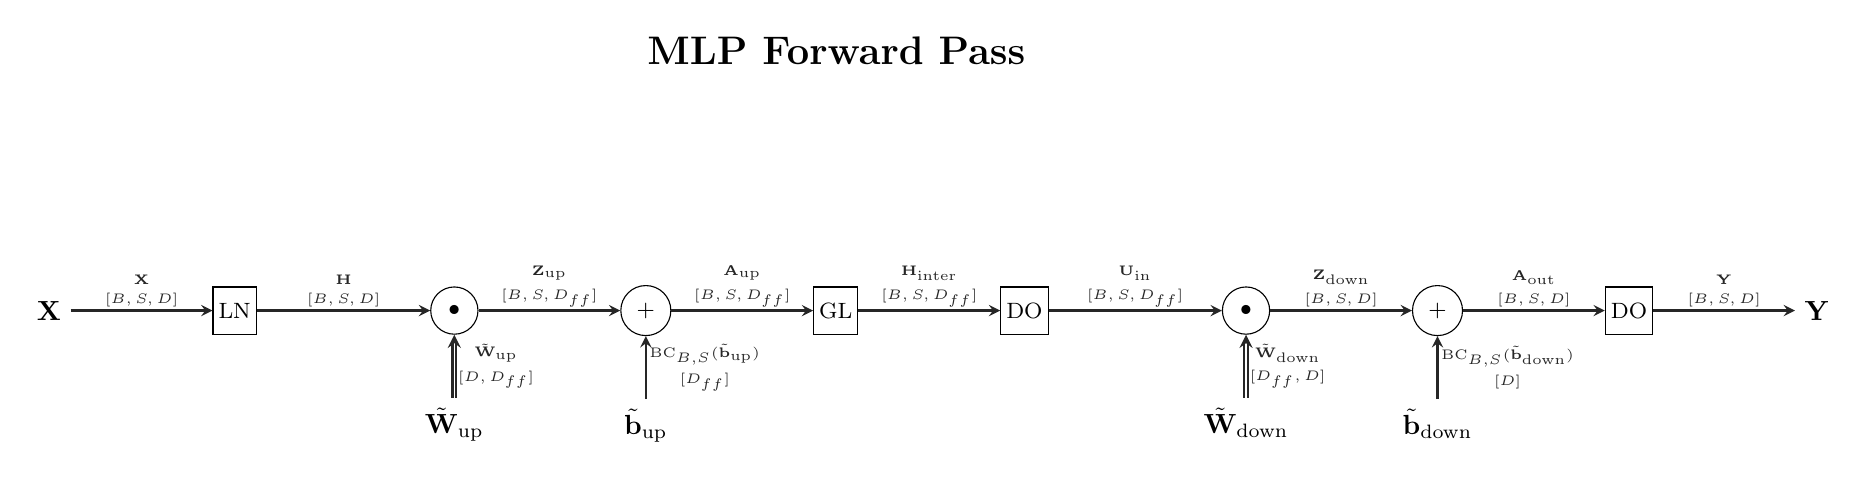
\begin{tikzpicture}[
    >=stealth,
    auxnode/.style={draw, rectangle, fill=white, minimum height=6mm, inner sep=2pt, font=\footnotesize, align=center},
    mulnode/.style={draw, circle, fill=white, minimum size=6mm, font=\footnotesize, align=center},
    addnode/.style={draw, circle, fill=white, minimum size=6mm, font=\footnotesize, align=center},
    sumnode/.style={draw, circle, fill=white, minimum size=6mm, font=\tiny, align=center},
    flow/.style={->, thick, black!85},
    flow2/.style={double, ->, thick, black!85},
    dimlabel/.style={font=\tiny, inner sep=1pt, align=center}
]
    \node[font=\Large\bfseries] at (10, 2.8) {MLP Forward Pass};

    \pgfmathsetmacro{\verticaloffset}{-0.5}

    \node            (MIn)   at (0,\verticaloffset) {$\mathbf{X}$};
    \node[auxnode]   (LN2)   [right=1.8cm of MIn] {LN};
    \node[mulnode]   (L1Mul) [right=2.2cm of LN2] {$\bullet$};
    \node            (Wup)   [below=0.8cm of L1Mul] {$\tilde{\mathbf{W}}_{\text{up}}$};
    \node[addnode]   (AddB1) [right=1.8cm of L1Mul] {+};
    \node            (Bup)   [below=0.8cm of AddB1] {$\tilde{\mathbf{b}}_{\text{up}}$};
    \node[auxnode]   (Act)   [right=1.8cm of AddB1] {GL};
    \node[auxnode]   (Drop1) [right=1.8cm of Act] {DO};
    \node[mulnode]   (L2Mul) [right=2.2cm of Drop1] {$\bullet$};
    \node            (Wdown) [below=0.8cm of L2Mul] {$\tilde{\mathbf{W}}_{\text{down}}$};
    \node[addnode]   (AddB2) [right=1.8cm of L2Mul] {+};
    \node            (Bdown) [below=0.8cm of AddB2] {$\tilde{\mathbf{b}}_{\text{down}}$};
    \node[auxnode]   (Drop2) [right=1.8cm of AddB2] {DO};
    \node            (MOut)  [right=1.8cm of Drop2] {$\mathbf{Y}$};

    \draw[flow] (MIn) -- (LN2) node[dimlabel, midway, above]{\shortstack{$\mathbf{X}$\\$[B,S,D]$}};
    \draw[flow] (LN2) -- (L1Mul) node[dimlabel, midway, above]{\shortstack{$\mathbf{H}$\\$[B,S,D]$}};
    \draw[flow2] (Wup) -- (L1Mul) node[dimlabel, midway, right]{\shortstack{$\tilde{\mathbf{W}}_{\text{up}}$\\$[D, D_{ff}]$}};
    \draw[flow] (L1Mul) -- (AddB1) node[dimlabel, midway, above]{\shortstack{$\mathbf{Z}_{\text{up}}$\\$[B,S,D_{ff}]$}};
    \draw[flow] (Bup) -- (AddB1) node[dimlabel, midway, right]{\shortstack{$\mathrm{BC}_{B,S}(\tilde{\mathbf{b}}_{\text{up}})$\\$[D_{ff}]$}};
    \draw[flow] (AddB1) -- (Act) node[dimlabel, midway, above]{\shortstack{$\mathbf{A}_{\text{up}}$\\$[B,S,D_{ff}]$}};
    \draw[flow] (Act) -- (Drop1) node[dimlabel, midway, above]{\shortstack{$\mathbf{H}_{\text{inter}}$\\$[B,S,D_{ff}]$}};
    \draw[flow] (Drop1) -- (L2Mul) node[dimlabel, midway, above]{\shortstack{$\mathbf{U}_{\text{in}}$\\$[B,S,D_{ff}]$}};
    \draw[flow2] (Wdown) -- (L2Mul) node[dimlabel, midway, right]{\shortstack{$\tilde{\mathbf{W}}_{\text{down}}$\\$[D_{ff}, D]$}};
    \draw[flow] (L2Mul) -- (AddB2) node[dimlabel, midway, above]{\shortstack{$\mathbf{Z}_{\text{down}}$\\$[B,S,D]$}};
    \draw[flow] (Bdown) -- (AddB2) node[dimlabel, midway, right]{\shortstack{$\mathrm{BC}_{B,S}(\tilde{\mathbf{b}}_{\text{down}})$\\$[D]$}};
    \draw[flow] (AddB2) -- (Drop2) node[dimlabel, midway, above]{\shortstack{$\mathbf{A}_{\text{out}}$\\$[B,S,D]$}};
    \draw[flow] (Drop2) -- (MOut) node[dimlabel, midway, above]{\shortstack{$\mathbf{Y}$\\$[B,S,D]$}};

\end{tikzpicture}%
}


\clearpage

\subsubsection{Backward Pass}
\noindent
\resizebox{\linewidth}{!}{%
\begin{tikzpicture}[
    >=stealth,
    auxnode/.style={draw, rectangle, fill=white, minimum height=6mm, inner sep=2pt, font=\footnotesize, align=center},
    mulnode/.style={draw, circle, fill=white, minimum size=6mm, font=\footnotesize, align=center},
    addnode/.style={draw, circle, fill=white, minimum size=6mm, font=\footnotesize, align=center},
    sumnode/.style={draw, circle, fill=white, minimum size=6mm, font=\tiny, align=center},
    flow_rev/.style={<-, thick, black!85},
    flow_dw/.style={->, thick, black!85},
    flow_act/.style={double, ->, thick, black!85},
    dimlabel/.style={font=\tiny, inner sep=1pt, align=center},
    gradlabel/.style={font=\tiny\bfseries, inner sep=1pt, align=center}
]
    \node[font=\Large\bfseries] at (5, 10) {MLP Backward Pass};

    \pgfmathsetmacro{\backwardoffset}{0.0}

    \node (d_MOut) at (12.6, \backwardoffset) {$\mathrm{d}\mathbf{Y}$};
    \node[auxnode] (d_Drop2) [left=1.8cm of d_MOut] {dDO};
    \draw[flow_rev] (d_Drop2) -- (d_MOut)
      node[dimlabel, midway, below]{\shortstack{$\mathrm{d}\mathbf{Y}$\\$[B,S,D]$}};

    \coordinate (split2) at ($(d_Drop2.west) + (-1.5cm, 0)$);
    \coordinate (branch_dUproj) at ($(split2) + (-1.2cm, 0)$);

    \node[sumnode] (d_SumB2) [above=0.8cm of split2] {$\sum_{B, S}$};
    \node (d_Bdown) [above=0.8cm of d_SumB2] {$\mathrm{d}\tilde{\mathbf{b}}_{\text{down}}$};
    \draw[flow_dw] (d_SumB2) -- (d_Bdown) node[dimlabel, midway, right]{$[D]$};

    \draw[flow_rev] (split2) -- (d_Drop2);
    \draw[flow_rev] (d_SumB2) -- (split2);

    \node[mulnode] (d_L2Mul_in) [left=2.2cm of split2] {$\bullet$};
    \draw[flow_rev] (d_L2Mul_in) -- (d_Drop2)
      node[gradlabel, midway, below]{\shortstack{$\mathrm{d}\mathbf{Z}_{\text{down}}=\mathrm{d}\mathbf{A}_{\text{out}}$\\$[B,S,D]$}};

    \node (W_down_T) [below=1.8cm of d_L2Mul_in] {$\tilde{\mathbf{W}}_{\text{down}}^{T}$};
    \draw[flow_act] (W_down_T.north) -- (d_L2Mul_in)
      node[dimlabel, midway, right]{$[D, D_{ff}]$};

    \coordinate (L2Mul_w_y) at ($(d_L2Mul_in) + (0, 3.5cm)$);
    \node[mulnode] (d_L2Mul_w) at (L2Mul_w_y) {$\bullet$};
    \node (d_Wdown) [above=0.8cm of d_L2Mul_w] {$\mathrm{d}\tilde{\mathbf{W}}_{\text{down}}$};
    \draw[flow_dw] (d_L2Mul_w) -- (d_Wdown) node[dimlabel, midway, right]{$[D_{ff}, D]$};

    \draw[flow_act] (branch_dUproj.north) |- (d_L2Mul_w.east);

    \node[auxnode] (Uin_T) at ($(d_L2Mul_w.west) + (-1.5cm, 0)$) {T};
    \draw[flow_dw] (Uin_T) -- (d_L2Mul_w)
      node[dimlabel, midway, below]{\shortstack{$\mathbf{U}_{\text{in}}^T$\\$[B, D_{ff}, S]$}};
    \node (Uin_aux) [left=1.8cm of Uin_T] {$\mathbf{U}_{\text{in}}$};
    \draw[flow_dw] (Uin_aux) -- (Uin_T) node[dimlabel, midway, above]{\shortstack{$[B,S,D_{ff}]$}};

    \node[auxnode] (d_Drop1) [left=1.8cm of d_L2Mul_in] {dDO};
    \draw[flow_rev] (d_Drop1) -- (d_L2Mul_in)
      node[dimlabel, midway, below]{\shortstack{$\mathrm{d}\mathbf{U}_{\text{in}}$\\$[B,S,D_{ff}]$}};

    \node[auxnode] (d_Act) [left=1.8cm of d_Drop1] {dGL};
    \draw[flow_rev] (d_Act) -- (d_Drop1)
      node[dimlabel, midway, below]{\shortstack{$\mathrm{d}\mathbf{H}_{\text{inter}}$\\$[B,S,D_{ff}]$}};

    \coordinate (split1) at ($(d_Act.west) + (-1.5cm, 0)$);
    \coordinate (branch_dHpre) at ($(split1) + (-1.2cm, 0)$);

    \node[sumnode] (d_SumB1) [above=0.8cm of split1] {$\sum_{B, S}$};
    \node (d_Bup) [above=0.8cm of d_SumB1] {$\mathrm{d}\tilde{\mathbf{b}}_{\text{up}}$};
    \draw[flow_dw] (d_SumB1) -- (d_Bup) node[dimlabel, midway, right]{$[D_{ff}]$};

    \draw[flow_rev] (split1) -- (d_Act);
    \draw[flow_rev] (d_SumB1) -- (split1);

    \node[mulnode] (d_L1Mul_in) [left=2.2cm of split1] {$\bullet$};
    \draw[flow_rev] (d_L1Mul_in) -- (d_Act)
      node[gradlabel, midway, below]{\shortstack{$\mathrm{d}\mathbf{Z}_{\text{up}}=\mathrm{d}\mathbf{A}_{\text{up}}$\\$[B,S,D_{ff}]$}};

    \node (W_up_T) [below=1.8cm of d_L1Mul_in] {$\tilde{\mathbf{W}}_{\text{up}}^{T}$};
    \draw[flow_act] (W_up_T.north) -- (d_L1Mul_in)
      node[dimlabel, midway, right]{$[D_{ff}, D]$};

    \coordinate (L1Mul_w_y) at ($(d_L1Mul_in) + (0, 3.5cm)$);
    \node[mulnode] (d_L1Mul_w) at (L1Mul_w_y) {$\bullet$};
    \node (d_Wup) [above=0.8cm of d_L1Mul_w] {$\mathrm{d}\tilde{\mathbf{W}}_{\text{up}}$};
    \draw[flow_dw] (d_L1Mul_w) -- (d_Wup) node[dimlabel, midway, right]{$[D, D_{ff}]$};

    \draw[flow_act] (branch_dHpre.north) |- (d_L1Mul_w.east);

    \node[auxnode] (Znorm_T) at ($(d_L1Mul_w.west) + (-1.5cm, 0)$) {T};
    \draw[flow_dw] (Znorm_T) -- (d_L1Mul_w)
      node[dimlabel, midway, below]{\shortstack{$\mathbf{H}^T$\\$[B, D, S]$}};
    \node (Znorm_aux) [left=1.8cm of Znorm_T] {$\mathbf{H}$};
    \draw[flow_dw] (Znorm_aux) -- (Znorm_T) node[dimlabel, midway, above]{\shortstack{$[B,S,D]$}};

    \node[auxnode] (d_LN2) [left=1.8cm of d_L1Mul_in] {dLN};
    \draw[flow_rev] (d_LN2) -- (d_L1Mul_in)
      node[dimlabel, midway, below]{\shortstack{$\mathrm{d}\mathbf{H}$\\$[B,S,D]$}};

    \node (d_MIn) [left=1.8cm of d_LN2] {$\mathrm{d}\mathbf{X}$};
    \draw[flow_rev] (d_MIn) -- (d_LN2)
      node[dimlabel, midway, below]{\shortstack{$\mathrm{d}\mathbf{X}$\\$[B,S,D]$}};
\end{tikzpicture}%
}


\clearpage

\subsubsection{Operations Summary}
\renewcommand{\arraystretch}{1.2}
\small
\begin{center}
\textbf{MLP (Feed-Forward) Block: Unified Table (Ops \& Data)}
\setlength{\tabcolsep}{6pt}
\begin{tabular}{lllll}
\hline
\textbf{Category} & \textbf{Symbol / Abbrev} & \textbf{Name} & \textbf{Shape / Type} & \textbf{Notes} \\
\hline
Ops & LN    & Layer Normalization   & op & Normalize per token (last dim $D$). \\
Ops & $\bullet$ & Linear (MatMul)   & op & Used for up/down projections. \\
Ops & $+$   & Bias Add              & op & Adds broadcast bias; $\mathrm{BC}_{B,S}(\cdot)$. \\
Ops & GL    & GELU (or activation)  & op & Nonlinearity on $D_{ff}$. \\
Ops & DO    & Dropout               & op & Training-time only (identity at inference). \\
Ops & T     & Transpose             & op & Used in weight-grad computations. \\
Ops & $\sum_{B,S}$ & Reduce-Sum     & op & Bias-grad accumulation over batch, seq. \\
\hline
Data & $\mathbf{X}$     & Input states         & $[B,S,D]$       & Block input. \\
Data & $\mathbf{H}$     & LN output            & $[B,S,D]$       & LN($\mathbf{X}$). \\
Data & $\tilde{\mathbf{W}}_{\text{up}}$   & Up weight     & $[D, D_{ff}]$ & First projection. \\
Data & $\tilde{\mathbf{b}}_{\text{up}}$   & Up bias       & $[D_{ff}]$    & Broadcast to $[B,S,D_{ff}]$. \\
Data & $\mathbf{Z}_{\text{up}}$           & Pre-activation & $[B,S,D_{ff}]$ & $H W_{\text{up}} + b_{\text{up}}$. \\
Data & $\mathbf{A}_{\text{up}}$           & Activated      & $[B,S,D_{ff}]$ & $f(\mathbf{Z}_{\text{up}})$. \\
Data & $\mathbf{H}_{\text{inter}}$        & Post-DO        & $[B,S,D_{ff}]$ & After Dropout. \\
Data & $\tilde{\mathbf{W}}_{\text{down}}$ & Down weight    & $[D_{ff},D]$  & Second projection. \\
Data & $\tilde{\mathbf{b}}_{\text{down}}$ & Down bias      & $[D]$         & Broadcast to $[B,S,D]$. \\
Data & $\mathbf{Z}_{\text{down}}$         & Linear output  & $[B,S,D]$     & $H_{\text{inter}} W_{\text{down}} + b_{\text{down}}$. \\
Data & $\mathbf{A}_{\text{out}}$          & Bias-added     & $[B,S,D]$     & Before dropout (out). \\
Data & $\mathbf{Y}$                       & Block output   & $[B,S,D]$     & After Dropout. \\
\hline
Data & $\text{d}\mathbf{Y}$                & Grad output    & $[B,S,D]$     & Incoming grad. \\
Data & $\text{d}\mathbf{Z}_{\text{down}}$  & Grad lin-out   & $[B,S,D]$     & Equals $d\mathbf{A}_{\text{out}}$. \\
Data & $\text{d}\mathbf{U}_{\text{in}}$    & Grad into down & $[B,S,D_{ff}]$& To weight/bias grads. \\
Data & $\text{d}\mathbf{Z}_{\text{up}}$    & Grad pre-act   & $[B,S,D_{ff}]$& Equals $d\mathbf{A}_{\text{up}}\cdot f'$. \\
Data & $\text{d}\mathbf{H}$                & Grad LN out    & $[B,S,D]$     & Into dLN. \\
Data & $\text{d}\mathbf{X}$                & Grad input     & $[B,S,D]$     & Block input grad. \\
Data & $\text{d}\tilde{\mathbf{W}}_{\text{up}}$   & Weight grad up   & $[D, D_{ff}]$ & From $H^T$ and $dZ_{\text{up}}$. \\
Data & $\text{d}\tilde{\mathbf{W}}_{\text{down}}$ & Weight grad down & $[D_{ff}, D]$ & From $U_{\text{in}}^T$ and $dZ_{\text{down}}$. \\
Data & $\text{d}\tilde{\mathbf{b}}_{\text{up}}$   & Bias grad up     & $[D_{ff}]$     & $\sum_{B,S} dZ_{\text{up}}$. \\
Data & $\text{d}\tilde{\mathbf{b}}_{\text{down}}$ & Bias grad down   & $[D]$          & $\sum_{B,S} dZ_{\text{down}}$. \\
\hline
\multicolumn{5}{l}{\textbf{Shape symbols: } $B$=batch,\; $S$=sequence,\; $D$=model dim,\; $D_{ff}$=FFN hidden dim (e.g., $4\times D$).}\\
\hline
\end{tabular}
\end{center}


\clearpage

% ---- 1.5 Output Projection ----
\subsection{Output Projection \& Loss Computation}

The final layer projects the hidden states to vocabulary logits and computes the cross-entropy loss.

\vspace{1cm}

\subsubsection{Forward Pass}

\noindent
\resizebox{\linewidth}{!}{%
\begin{tikzpicture}[
  >=stealth,
  auxnode/.style={draw, rectangle, fill=white, minimum height=6mm, inner sep=2pt, font=\footnotesize, align=center},
  mulnode/.style={draw, circle, fill=white, minimum size=6mm, font=\footnotesize, align=center},
  addnode/.style={draw, circle, fill=white, minimum size=6mm, font=\footnotesize, align=center},
  sumnode/.style={draw, circle, fill=white, minimum size=6mm, font=\tiny, align=center},
  flow/.style={->, thick, black!85},
  flow2/.style={double, ->, thick, black!85},
  dimlabel/.style={font=\tiny, inner sep=1pt, align=center}
]

% From Transformer output
\node            (H)     at (0,-2) {$\mathbf{A}_{\text{out}}$};

% LM head
\node[mulnode]   (LMmul) [right=2.2cm of H] {$\bullet$};
\node            (Wlm)   [align=center, below=0.9cm of LMmul] {$\widetilde{\mathbf{W}}_{\text{lm}}$\\$=\mathbf{E}^{T}$};
\node[addnode]   (AddB)  [right=1.8cm of LMmul] {+};
\node            (blm)   [below=0.9cm of AddB] {$\widetilde{\mathbf{b}}_{\text{lm}}$};

% Softmax → Prob
\node[auxnode]   (SM)    [right=1.8cm of AddB] {S};

\node[auxnode] (ARG)  [right=4.0cm of SM] {ARG};
% Midpoint of SM→P edge (for CE tap)
\coordinate (MidSP) at ($(SM)!0.5!(ARG)$);

% CE node placed below the SM→P edge
\node[auxnode]   (CE)    [below=1.6cm of MidSP] {CE};
\node            (Y)     [right=0.9cm of CE] {$\mathbf{Y_\text{targets}}$};
\node            (Loss)  [align=center, below=1.8cm of CE] {$\mathcal{L}$\\ (mean over $B,S$)};

% Flows
\draw[flow]  (H) -- (LMmul) node[dimlabel, midway, above]{\shortstack{$[B,S,D]$}};
\draw[flow2] (Wlm) -- (LMmul) node[dimlabel, midway, right]{\shortstack{$[D,V]$}};
\draw[flow]  (LMmul) -- (AddB) node[dimlabel, midway, above]{\shortstack{$\mathbf{Z}_{\text{lin}}$\\$[B,S,V]$}};
\draw[flow]  (blm) -- (AddB)   node[dimlabel, midway, right]{\shortstack{$\text{BC}_{B,S}(\widetilde{\mathbf{b}}_{\text{lm}})$\\$[V]$}};
\draw[flow]  (AddB) -- (SM)    node[dimlabel, midway, above]{\shortstack{\textbf{Z\textsubscript{bias}}\\ $[B,S,V]$}};

% Tap the SM→P edge downward into CE
\draw[flow]  (MidSP) -- (CE);
% Targets into CE
\draw[flow]  (Y) -- (CE)  node[dimlabel, midway, above]{\shortstack{targets\\$[B,S]$}};
% Loss goes WEST (left) from CE
\draw[flow]  (CE) -- (Loss);

\node (YhatG) [right=1.8cm of ARG] {$\hat{\mathbf{Y}}_{\text{greedy}}$};
\draw[flow] (SM) -- (ARG)
  node[dimlabel, pos=0.35, above]{\shortstack{$\mathbf{P}$\\$[B,S,V]$}};
\draw[flow] (ARG) -- (YhatG)
  node[dimlabel, midway, above]{\shortstack{token ids\\$[B,S]$}};

% Optional: top-k (or nucleus) sampling path
\node[auxnode] (TopK) [above=1.4cm of ARG] {TOP-$k$};
\node          (YhatS) [right=1.8cm of TopK] {$\hat{\mathbf{Y}}_{\text{sample}}$};
\draw[flow] (MidSP) |- (TopK);
\draw[flow] (TopK) -- (YhatS)
  node[dimlabel, midway, above]{\shortstack{token ids\\$[B,S]$}};

\node[font=\large\bfseries] at (9.2,1.8) {Token Generation \& Loss (Forward)};
\end{tikzpicture}%
}


\clearpage

\subsubsection{Backward Pass}
\noindent
\resizebox{0.8\linewidth}{!}{%
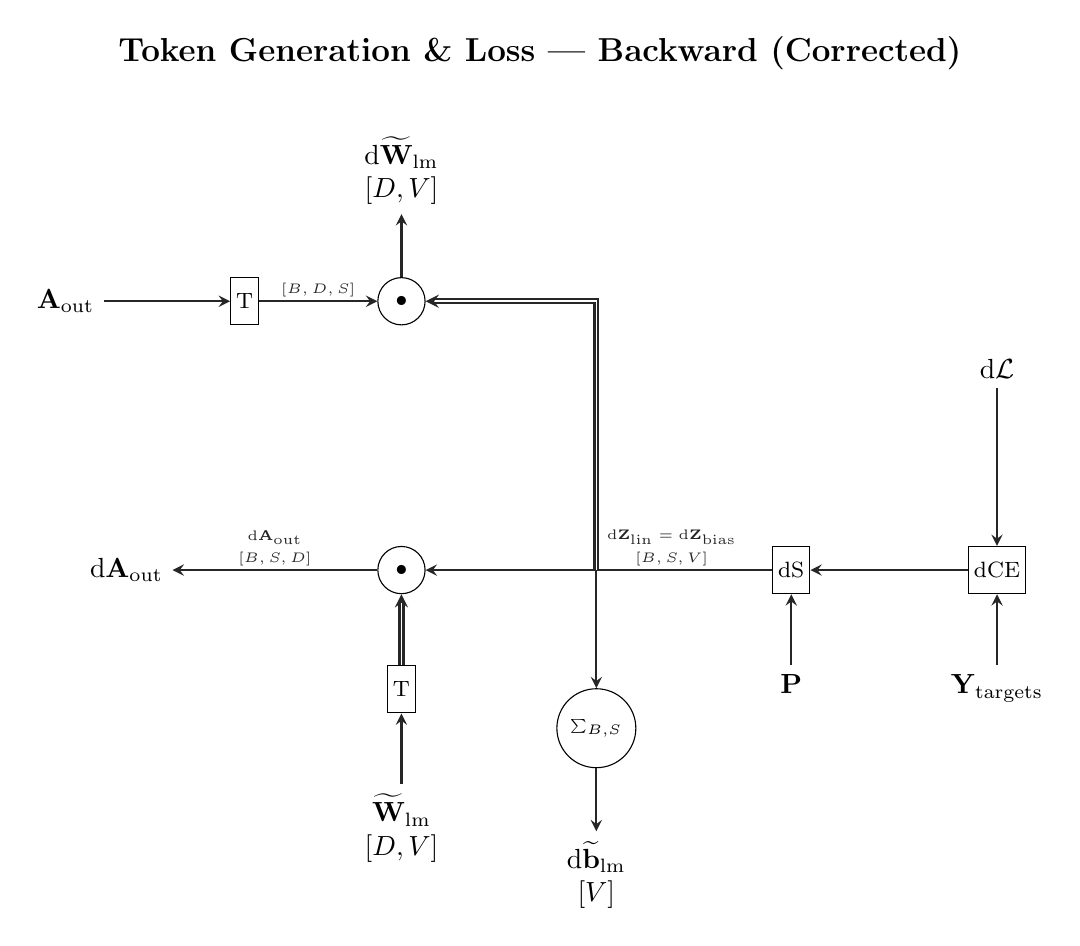
\begin{tikzpicture}[
  >=stealth,
  auxnode/.style={draw, rectangle, fill=white, minimum height=6mm, inner sep=2pt, font=\footnotesize, align=center},
  mulnode/.style={draw, circle, fill=white, minimum size=6mm, font=\footnotesize, align=center},
  addnode/.style={draw, circle, fill=white, minimum size=6mm, font=\footnotesize, align=center},
  sumnode/.style={draw, circle, fill=white, minimum size=6mm, font=\tiny, align=center},
  flow/.style={<-, thick, black!85},
  flow2/.style={double, <-, thick, black!85},
  fwd/.style={->, thick, black!85},
  gradflow/.style={->, thick, black!85},
  dimlabel/.style={font=\tiny, inner sep=1pt, align=center}
]

% Start from dL
\node           (dL)    at (18,0) {$\text{d}\mathcal{L}$};
\node[auxnode]  (dCE)   [below=2.0cm of dL] {dCE};
\node           (Y)     [below=0.9cm of dCE] {$\mathbf{Y_\text{targets}}$};

% Softmax backward
\node[auxnode]  (dS)   [left=2.0cm of dCE] {dS};
\node           (P)     [below=0.9cm of dS] {$\mathbf{P}$};

% Logits (Linear Projection) backprop node
\node[mulnode]  (backMul) [left=4.4cm of dS] {$\bullet$};
\node[auxnode]  (T_Wlm)   [below=0.9cm of backMul] {T};
\node           (Wlm)     [align=center, below=0.9cm of T_Wlm] {$\widetilde{\mathbf{W}}_{\text{lm}}$\\$[D,V]$};

\coordinate (B_split) at ($(backMul)!0.5!(dS)$);

% SUM node for Bias gradient
\node[sumnode]  (SumB) [below=1.5cm of B_split] {$\sum_{B,S}$};
\node           (db)   [align=center, below=0.8cm of SumB] {$\text{d}\widetilde{\mathbf{b}}_{\text{lm}}$\\$[V]$};

% dW calc
\node[mulnode]  (dWmul) [above=2.8cm of backMul] {$\bullet$};
\node[auxnode]  (TAout) [left=1.5cm of dWmul] {T};
\node           (Aout)  [left=1.6cm of TAout] {$\mathbf{A}_{\text{out}}$};
\node           (dW)    [align=center, above=0.8cm of dWmul] {$\text{d}\widetilde{\mathbf{W}}_{\text{lm}}$\\$[D,V]$};

% Back to Transformer
\node           (dH)    [left=2.6cm of backMul] {$\text{d}\mathbf{A}_{\text{out}}$};

% Flows
\draw[flow] (dCE) -- (dL);
\draw[fwd]  (Y) -- (dCE);
\draw[flow] (dS) -- (dCE);
\draw[fwd]  (P) -- (dS);

% Bias grad
\draw[gradflow] (B_split) -- (SumB.north);
\draw[gradflow] (SumB) -- (db);

% Linear projection backprop
\draw[flow] (backMul) -- (dS)
  node[dimlabel, pos=0.71, above]{\shortstack{$\text{d}\mathbf{Z}_{\text{lin}}=\text{d}\mathbf{Z}_{\text{bias}}$\\$[B,S,V]$}};
\draw[flow2] (backMul) -- (T_Wlm);
\draw[fwd]   (Wlm) -- (T_Wlm);
\draw[flow]  (dH) -- (backMul) node[dimlabel, midway, above]{\shortstack{$\text{d}\mathbf{A}_{\text{out}}$\\$[B,S,D]$}};

% dW calculation
\draw[gradflow] (dWmul) -- (dW);
\draw[fwd]  (Aout) -- (TAout);
\draw[fwd]  (TAout) -- (dWmul) node[dimlabel, midway, above]{\shortstack{$[B,D,S]$}};
\draw[flow2] (dWmul) -| (B_split);

\node[font=\large\bfseries, anchor=south]
  at ([yshift=6mm]current bounding box.north) {Token Generation \& Loss — Backward (Corrected)};
\end{tikzpicture}%
}


\clearpage

\subsubsection{Operations Summary}
\renewcommand{\arraystretch}{1.2}
\small

% -------- Operations (Ops) --------
\begin{center}
\textbf{Operations (Ops)}
\begin{tabular}{llll}
\hline
\textbf{Abbrev} & \textbf{Name} & \textbf{Type / Shape} & \textbf{Notes} \\
\hline
S     & Softmax                     & op            & Over vocab axis $V$; outputs probabilities $\mathbf{P}$. \\
CE    & Cross-Entropy               & op            & Usually \emph{sparse} CE consuming label indices $\mathbf{Y}$. \\
ARG   & Argmax (greedy)             & op            & $\operatorname*{argmax}_V$ to get token ids (no gradient). \\
TOP-$k$ & Top-$k$ / sampling        & op            & Optional decoding path; no gradient. \\
T     & Transpose                   & op            & E.g., $\widetilde{\mathbf{W}}_{\text{lm}}^{T} \in \mathbb{R}^{V\times D}$. \\
$\mathrm{BC}_{B,S}(\cdot)$ & Broadcast & op       & Expand $[V] \!\to\! [B,S,V]$ for bias add. \\
dS    & Softmax backward            & op            & With CE: $\mathrm{d}\mathbf{Z}_{\text{bias}}=\mathbf{P}-\text{onehot}(\mathbf{Y})$. \\
dAddB & Addition (Bias) backward    & op            & Sends $\mathrm{d}\mathbf{Z}_{\text{bias}}$ to matmul and $\sum_{B,S}$.\\
$\sum_{B,S}$ & Summation            & op            & Yields $\mathrm{d}\widetilde{\mathbf{b}}_{\text{lm}}$.\\
\hline
\end{tabular}
\end{center}

\vspace{0.8em}

% -------- Data Tensors (Values) --------
\begin{center}
\textbf{Data Tensors (Values)}
\begin{tabular}{lllp{0.46\linewidth}}
\hline
\textbf{Symbol} & \textbf{Name} & \textbf{Shape} & \textbf{Notes} \\
\hline
$\mathbf{A}_{\text{out}}$ & Transformer output (hidden) & $[B,S,D]$ & Final hidden from the Transformer block(s). \\
$\widetilde{\mathbf{W}}_{\text{lm}}$ & LM head weight (tied) & $[D,V]$ & Typically tied to $\mathbf{E}^{T}$. \\
$\widetilde{\mathbf{b}}_{\text{lm}}$ & LM head bias           & $[V]$    & Broadcast-added over $[B,S,V]$. \\
$\mathbf{Z}_{\text{lin}}$ & Logits (linear output) & $[B,S,V]$ & $\mathbf{A}_{\text{out}}\widetilde{\mathbf{W}}_{\text{lm}}$. \\
$\mathbf{Z}_{\text{bias}}$ & Logits (final/Softmax input) & $[B,S,V]$ & $\mathbf{Z}_{\text{lin}}+\widetilde{\mathbf{b}}_{\text{lm}}$. \\
$\mathbf{P}$ & Probabilities                     & $[B,S,V]$ & $\mathrm{softmax}(\mathbf{Z}_{\text{bias}})$. \\
$\mathbf{Y}$ & Target token ids                  & $[B,S]$   & Ground-truth indices (sparse labels). \\
$\mathcal{L}$ & Loss                              & scalar or $[B,S]$ & Typically mean over $B,S$. \\
$\mathrm{d}\mathcal{L}$ & Loss gradient          & scalar-grad & Starting signal for backward pass. \\
$\mathrm{d}\mathbf{Z}_{\text{bias}}$  & Final Logits gradient  & $[B,S,V]$  & From CE+Softmax: $\mathbf{P}-\text{onehot}(\mathbf{Y})$. \\
$\mathrm{d}\mathbf{Z}_{\text{lin}}$ & Linear output grad & $[B,S,V]$ & Same as $\mathrm{d}\mathbf{Z}_{\text{bias}}$. \\
$\mathrm{d}\widetilde{\mathbf{W}}_{\text{lm}}$ & LM weight grad & $[D,V]$ & $=\mathbf{A}_{\text{out}}^{T}\mathrm{d}\mathbf{Z}_{\text{lin}}$. \\
$\mathrm{d}\widetilde{\mathbf{b}}_{\text{lm}}$ & LM bias grad & $[V]$ & $=\sum_{B,S}\mathrm{d}\mathbf{Z}_{\text{bias}}$. \\
$\mathrm{d}\mathbf{A}_{\text{out}}$ & Hidden grad & $[B,S,D]$  & $=\mathrm{d}\mathbf{Z}_{\text{lin}}\,\widetilde{\mathbf{W}}_{\text{lm}}^{T}$. \\
\hline
\multicolumn{4}{l}{\textbf{Shapes:}\ $B$=batch,\ $S$=sequence length,\ $D$=hidden dim,\ $V$=vocab size.} \\
\hline
\end{tabular}
\end{center}


\clearpage

% ============================================================
% CHAPTER 2: TENSOR PARALLELISM (TP)
% ============================================================
\section{Tensor Parallelism (TP)}

\textit{[This chapter will cover Tensor Parallelism implementation details]}

\subsection{TP Overview}
\textit{[To be added]}
\resizebox{\linewidth}{!}{%
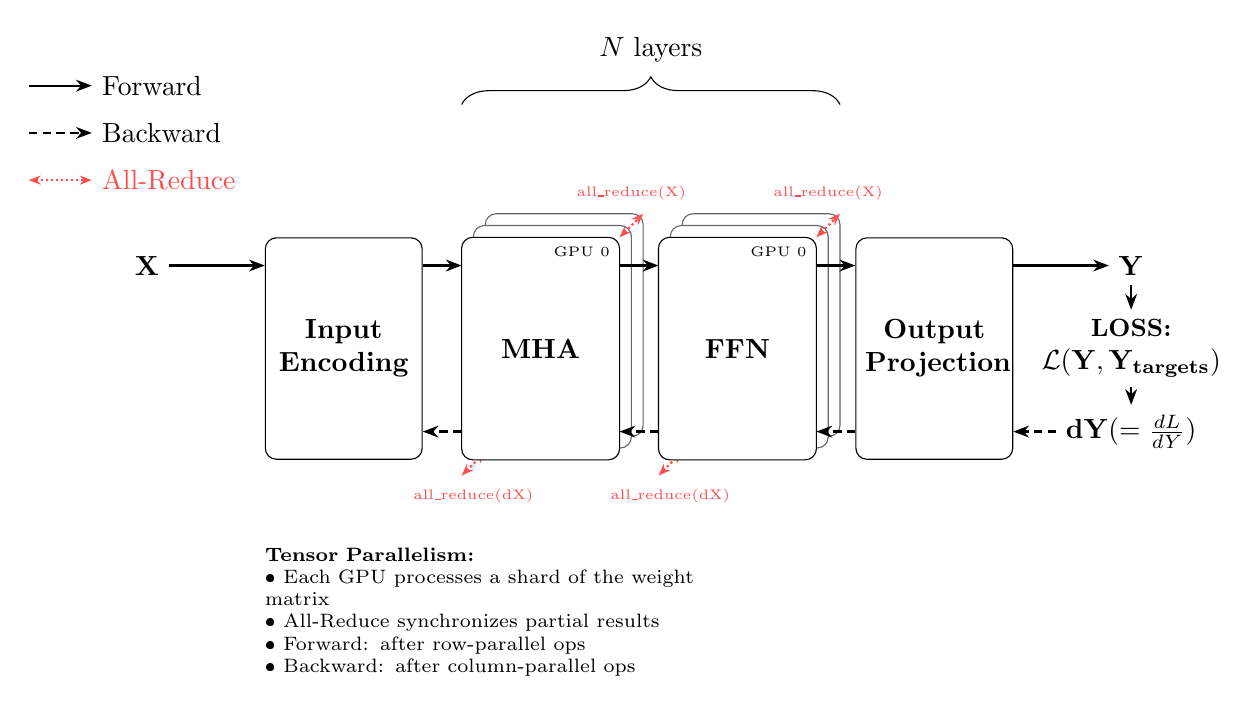
\begin{tikzpicture}[
    node distance=2.5cm,
    >=stealth,
    block/.style={rectangle, draw=black, fill=white, text width=5em, text centered, rounded corners, minimum height=8em, font=\bfseries},
    blockstack/.style={rectangle, draw=black!60, fill=white, text width=5em, text centered, rounded corners, minimum height=8em},
    forward/.style={-{Stealth[length=2mm]}, thick, black},
    backward/.style={-{Stealth[length=2mm]}, thick, black, densely dashed},
    allreduce/.style={{Stealth[length=1.5mm]}-{Stealth[length=1.5mm]}, thick, red!70, densely dotted},
    io/.style={text centered, font=\bfseries}
]
    % Title
    % \node[font=\Large\bfseries] at (10, 6) {Transformer Overall Flow (TP with 3 GPUs)};

    % Forward path nodes (horizontal)
    \node (input) [io] {$\mathbf{X}$};
    \node (encoding) [block, right of=input, yshift=-3em] {Input\\Encoding};

    % MHA blocks (3 stacked) - GPU 2 (back)
    \node (mha3) [blockstack, right of=encoding, xshift=0.3cm, yshift=0.3cm] {};
    % MHA blocks (3 stacked) - GPU 1 (middle)
    \node (mha2) [blockstack, right of=encoding, xshift=0.15cm, yshift=0.15cm] {};
    % MHA blocks (3 stacked) - GPU 0 (front)
    \node (mha) [block, right of=encoding] {MHA};

    % Small GPU labels for MHA
    \node[font=\tiny, anchor=north east] at (mha.north east) {GPU 0};

    % FFN blocks (3 stacked) - GPU 2 (back)
    \node (mlp3) [blockstack, right of=mha, xshift=0.3cm, yshift=0.3cm] {};
    % FFN blocks (3 stacked) - GPU 1 (middle)
    \node (mlp2) [blockstack, right of=mha, xshift=0.15cm, yshift=0.15cm] {};
    % FFN blocks (3 stacked) - GPU 0 (front)
    \node (mlp) [block, right of=mha] {FFN};

    % Small GPU labels for FFN
    \node[font=\tiny, anchor=north east] at (mlp.north east) {GPU 0};

    \node (output) [block, right of=mlp] {Output\\Projection};
    \node (pred) [io, right of=output, yshift=3em] {$\mathbf{Y}$};
    \node (loss) [align=center, io, right of=output] {\small LOSS:\\$\mathcal{L}(\mathbf{Y,Y_\text{targets}})$};
    \node (gradient) [io, right of=output, yshift=-3em] {$\mathbf{dY}(=\frac{dL}{dY})$};

    % All-Reduce arrows (Backward drawn first, then blocks, then Forward on top)
    % Backward All-Reduce - FFN (left-bottom corner, lower position)
    \draw [allreduce] ([yshift=-0.2cm]mlp.south west) -- ([xshift=0.3cm, yshift=0.1cm]mlp.south west);
    \node[font=\tiny, red!70, anchor=north] at ([xshift=0.15cm, yshift=-0.25cm]mlp.south west) {all\_reduce(dX)};

    % Backward All-Reduce - MHA (left-bottom corner, lower position)
    \draw [allreduce] ([yshift=-0.2cm]mha.south west) -- ([xshift=0.3cm, yshift=0.1cm]mha.south west);
    \node[font=\tiny, red!70, anchor=north] at ([xshift=0.15cm, yshift=-0.25cm]mha.south west) {all\_reduce(dX)};

    % Redraw blocks to cover backward All-Reduce arrows
    \draw [draw=black!60, fill=white, rounded corners] (mha3.south west) rectangle (mha3.north east);
    \draw [draw=black!60, fill=white, rounded corners] (mha2.south west) rectangle (mha2.north east);
    \draw [draw=black, fill=white, rounded corners, line width=0.4pt] (mha.south west) rectangle (mha.north east);
    \node[font=\bfseries] at (mha.center) {MHA};
    \node[font=\tiny, anchor=north east] at (mha.north east) {GPU 0};

    \draw [draw=black!60, fill=white, rounded corners] (mlp3.south west) rectangle (mlp3.north east);
    \draw [draw=black!60, fill=white, rounded corners] (mlp2.south west) rectangle (mlp2.north east);
    \draw [draw=black, fill=white, rounded corners, line width=0.4pt] (mlp.south west) rectangle (mlp.north east);
    \node[font=\bfseries] at (mlp.center) {FFN};
    \node[font=\tiny, anchor=north east] at (mlp.north east) {GPU 0};

    % Forward All-Reduce - MHA (right-top corner) - drawn after blocks to appear on top
    \draw [allreduce] (mha.north east) -- ([xshift=0.3cm, yshift=0.3cm]mha.north east);
    \node[font=\tiny, red!70, anchor=south] at ([xshift=0.15cm, yshift=0.35cm]mha.north east) {all\_reduce(X)};

    % Forward All-Reduce - FFN (right-top corner) - drawn after blocks to appear on top
    \draw [allreduce] (mlp.north east) -- ([xshift=0.3cm, yshift=0.3cm]mlp.north east);
    \node[font=\tiny, red!70, anchor=south] at ([xshift=0.15cm, yshift=0.35cm]mlp.north east) {all\_reduce(X)};

    % Forward arrows (upper part of blocks)
    \draw [forward] (input) -- ([yshift=3em]encoding.west);
    \draw [forward] ([yshift=3em]encoding.east) -- ([yshift=3em]mha.west);
    \draw [forward] ([yshift=3em]mha.east) -- ([yshift=3em]mlp.west);
    \draw [forward] ([yshift=3em]mlp.east) -- ([yshift=3em]output.west);
    \draw [forward] ([yshift=3em]output.east) -- (pred);
    \draw [forward] (pred) -- (loss);
    \draw [backward] (loss) -- (gradient);

    % Backward arrows (lower part of blocks)
    \draw [backward] (gradient) -- ([yshift=-3em]output.east);
    \draw [backward] ([yshift=-3em]output.west) -- ([yshift=-3em]mlp.east);
    \draw [backward] ([yshift=-3em]mlp.west) -- ([yshift=-3em]mha.east);
    \draw [backward] ([yshift=-3em]mha.west) -- ([yshift=-3em]encoding.east);

    % Brace for layer repetition (horizontal - using mlp with x offset to match mlp3)
    \draw[decorate, decoration={brace, amplitude=10pt}]
        ([yshift=4.8em]mha.north west) -- ([xshift=0.3cm, yshift=4.8em]mlp.north east)
        node[midway, above=12pt, font=\normalsize] {$N$ layers};

    % Labels (Legend)
    \coordinate (legend) at ([xshift=-1.5cm, yshift=6.5em]input);
    \draw[forward] (legend) -- ++(0.8,0) node[right, font=\normalsize] {Forward};
    \draw[backward] ([yshift=-0.6cm]legend) -- ++(0.8,0) node[right, font=\normalsize] {Backward};
    \draw[allreduce] ([yshift=-1.2cm]legend) -- ++(0.8,0) node[right, font=\normalsize] {All-Reduce};

    % TP explanation
    \node[font=\scriptsize, align=left, text width=6cm] at ([xshift=2cm, yshift=-5.5em]encoding.south) {
        \textbf{Tensor Parallelism:}\\
        • Each GPU processes a shard of the weight matrix\\
        • All-Reduce synchronizes partial results\\
        • Forward: after row-parallel ops\\
        • Backward: after column-parallel ops
    };

\end{tikzpicture}%
}

\clearpage


\subsection{Forward Pass}

In the tensor-parallel setting, the multi-head attention is distributed across $N_T$ devices (GPUs). The notation used in the diagram is defined as follows:
\begin{itemize}
    \item $N_H$: Total number of attention heads (global)
    \item $N_T$: Tensor parallelism degree (number of devices)
    \item $N_{HN}$: Number of heads per device (local), where $N_{HN} = \frac{N_H}{N_T}$
\end{itemize}

Each device processes $N_{HN}$ heads independently. The weight matrices $\widetilde{\mathbf{W}}_Q$, $\widetilde{\mathbf{W}}_K$, $\widetilde{\mathbf{W}}_V$, and $\widetilde{\mathbf{W}}_O$ are column-partitioned across devices, with each device holding a $[D, N_{HN} \cdot D_h]$ slice of the original $[D, D]$ matrix.



\resizebox{\linewidth}{!}{%
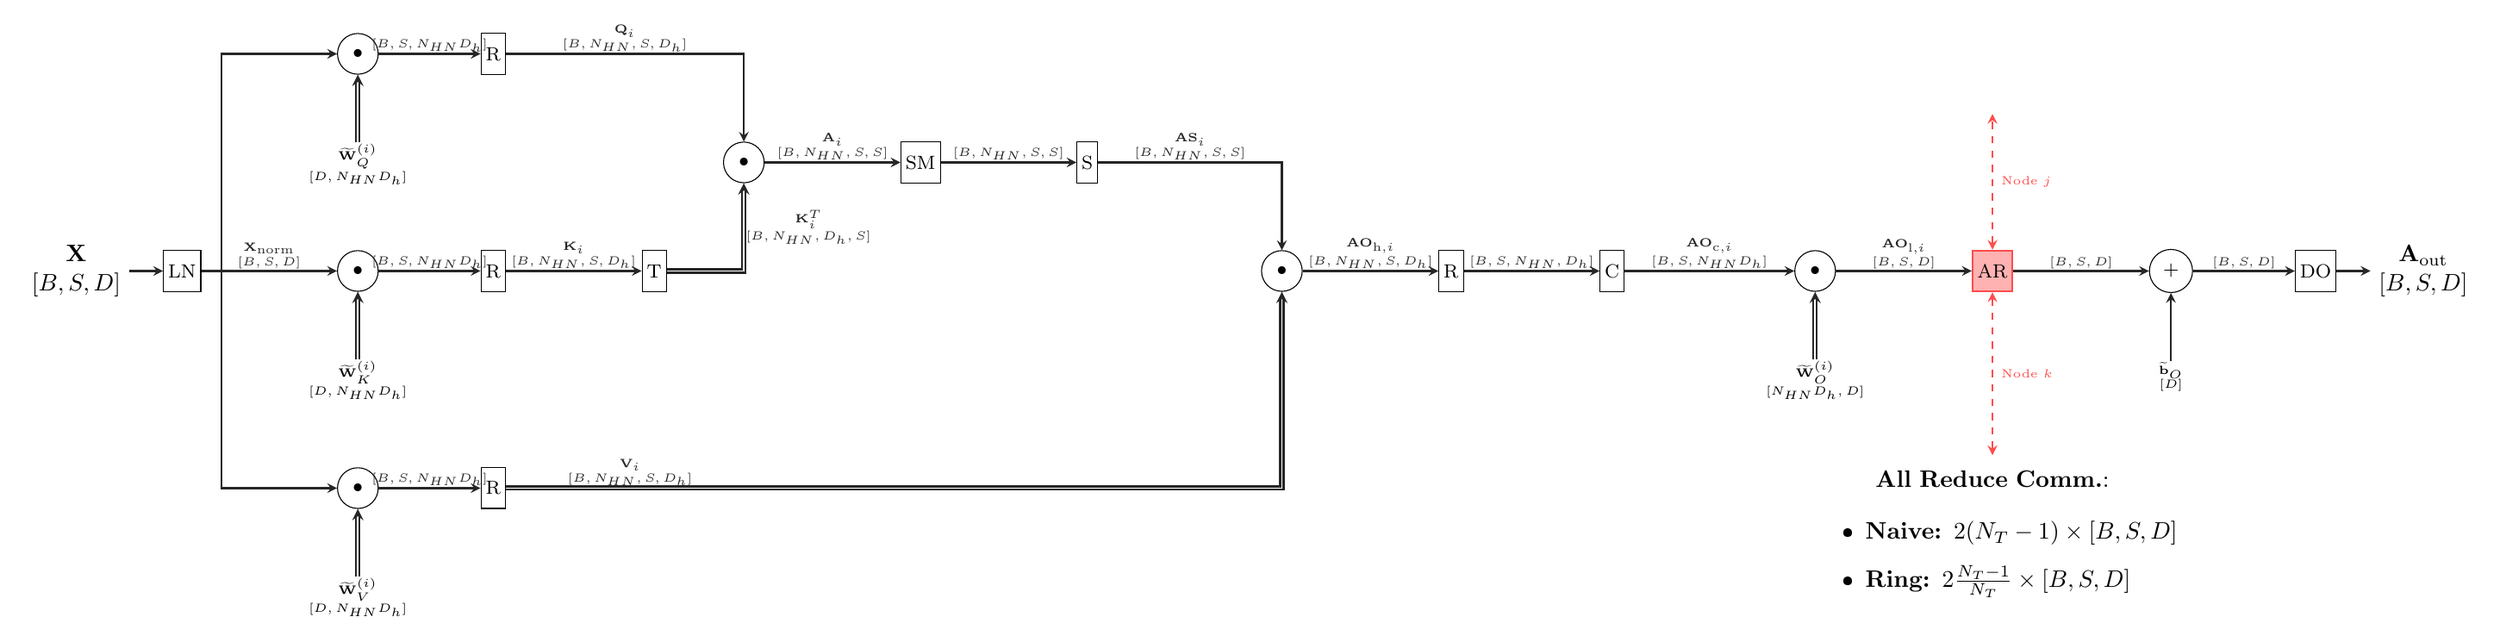
\begin{tikzpicture}[
  every node/.style={transform shape},
  >=stealth,
  auxnode/.style={draw, rectangle, fill=white, minimum height=6mm, inner sep=2pt, font=\footnotesize, align=center},
  mulnode/.style={draw, circle, fill=white, minimum size=6mm, font=\footnotesize, align=center},
  addnode/.style={draw, circle, fill=white, minimum size=6mm, font=\footnotesize, align=center},
  allreduce/.style={draw, rectangle, fill=red!30, minimum height=6mm, inner sep=2pt, font=\footnotesize, align=center, thick, draw=red!70},
  flow/.style={->, thick, black!85},
  flow2/.style={->, double, thick, black!85},
  commflow/.style={<->, thick, red!70, dashed},
  dimlabel/.style={font=\tiny, inner sep=0.5pt, align=center}
]
% \node[font=\Large\bfseries] at (9, 4.5) {Multi-Head Attention Forward Pass (Node $i$)};

\node (Input) at (0.5, 0) [align=center] {$\mathbf{X}$\\$[B,S,D]$};
\node[auxnode] (LN) [right=0.5cm of Input] {LN};

\node[mulnode] (Proj_Q) [right=2.0cm of LN, yshift=3.2cm] {$\bullet$};
\node[auxnode] (R_Q) [right=1.5cm of Proj_Q] {R};

\node[mulnode] (Proj_K) [right=2.0cm of LN, yshift=0cm] {$\bullet$};
\node[auxnode] (R_K) [right=1.5cm of Proj_K] {R};

\node[mulnode] (Proj_V) [right=2.0cm of LN, yshift=-3.2cm] {$\bullet$};
\node[auxnode] (R_V) [right=1.5cm of Proj_V] {R};

\node[dimlabel] (WQ) [align=center, below=1.0cm of Proj_Q] {$\widetilde{\mathbf{W}}_{Q}^{(i)}$\\$[D,N_{HN}D_h]$};
\node[dimlabel] (WK) [align=center, below=1.0cm of Proj_K] {$\widetilde{\mathbf{W}}_{K}^{(i)}$\\$[D,N_{HN}D_h]$};
\node[dimlabel] (WV) [align=center, below=1.0cm of Proj_V] {$\widetilde{\mathbf{W}}_{V}^{(i)}$\\$[D,N_{HN}D_h]$};

\node[auxnode] (T_K) [right=2.0cm of R_K] {T};
\node[mulnode] (QK) [right=3.2cm of R_Q, yshift=-1.6cm] {$\bullet$};
\node[auxnode] (SM) [right=2.0cm of QK] {SM};
\node[auxnode] (Soft) [right=2.0cm of SM] {S};
\node[mulnode] (PV) [right=2.4cm of Soft, yshift=-1.6cm] {$\bullet$};

\node[auxnode] (R_Merge) [right=2.0cm of PV] {R};
\node[auxnode] (Cat) [right=2.0cm of R_Merge] {C};

\node[mulnode] (OProj) [right=2.5cm of Cat] {$\bullet$};
\node[dimlabel] (WO_FWD) [align=center, below=1.0cm of OProj] {$\widetilde{\mathbf{W}}_{O}^{(i)}$\\$[N_{HN}D_h,D]$};
\node[allreduce] (AR) [right=2.0cm of OProj] {AR};
\node[
  align=center,
  below=2.5cm of AR,
  text width=5.5cm % 적당한 값으로 조정
] (AR_info) {%
  \textbf{All Reduce Comm.}:\\[2pt]
  \begin{itemize}
    \item \textbf{Naive:} $2(N_T-1) \times [B,S,D]$
    \item \textbf{Ring:} $2\frac{N_T-1}{N_T} \times [B,S,D]$
  \end{itemize}
};
\node[addnode] (AddB) [right=2.0cm of AR] {+};
\node[dimlabel] (BO) [align=center, below=1.0cm of AddB] {$\widetilde{\mathbf{b}}_{O}$\\$[D]$};
\node[auxnode] (Drop) [right=1.5cm of AddB] {DO};
\node (Aout) [align=center, right=0.5cm of Drop] {$\mathbf{A}_{\text{out}}$\\$[B,S,D]$};

\draw[flow] (Input) -- (LN);

\draw[flow] (LN.east) -- ++(0.3,0) |- (Proj_Q.west);
\draw[flow] (LN) -- (Proj_K.west) node[dimlabel, midway, above]{$\mathbf{X}_{\text{norm}}$\\$[B,S,D]$};
\draw[flow] (LN.east) -- ++(0.3,0) |- (Proj_V.west);

\draw[flow2] (WQ) -- (Proj_Q);
\draw[flow2] (WK) -- (Proj_K);
\draw[flow2] (WV) -- (Proj_V);

\draw[flow] (Proj_Q) -- (R_Q) node[dimlabel, midway, above]{$[B,S,N_{HN}D_h]$};
\draw[flow] (Proj_K) -- (R_K) node[dimlabel, midway, above]{$[B,S,N_{HN}D_h]$};
\draw[flow] (Proj_V) -- (R_V) node[dimlabel, midway, above]{$[B,S,N_{HN}D_h]$};

\draw[flow] (R_Q) -| (QK) node[dimlabel, near start, above]{$\mathbf{Q}_i$\\$[B,N_{HN},S,D_h]$};
\draw[flow] (R_K) -- (T_K) node[dimlabel, midway, above]{$\mathbf{K}_i$\\$[B,N_{HN},S,D_h]$};
\draw[flow2] (T_K) -| (QK) node[dimlabel, near end, right]{$\mathbf{K}_i^{T}$\\$[B,N_{HN},D_h,S]$};

\draw[flow] (QK) -- (SM) node[dimlabel, midway, above]{$\mathbf{A}_i$\\$[B,N_{HN},S,S]$};
\draw[flow] (SM) -- (Soft) node[dimlabel, midway, above]{$[B,N_{HN},S,S]$};
\draw[flow] (Soft) -| (PV) node[dimlabel, near start, above]{$\mathbf{AS}_i$\\$[B,N_{HN},S,S]$};
\draw[flow2] (R_V) -| (PV) node[dimlabel, pos=0.08, above]{$\mathbf{V}_i$\\$[B,N_{HN},S,D_h]$};

\draw[flow] (PV) -- (R_Merge) node[dimlabel, midway, above]{$\mathbf{AO}_{\text{h},i}$\\$[B,N_{HN},S,D_h]$};
\draw[flow] (R_Merge) -- (Cat) node[dimlabel, midway, above]{$[B,S,N_{HN},D_h]$};
\draw[flow] (Cat) -- (OProj) node[dimlabel, midway, above]{$\mathbf{AO}_{\text{c},i}$\\$[B,S,N_{HN}D_h]$};
\draw[flow2] (WO_FWD) -- (OProj);
\draw[flow] (OProj) -- (AR) node[dimlabel, midway, above]{$\mathbf{AO}_{\text{l},i}$\\$[B,S,D]$};

% All-Reduce communication arrows
\draw[commflow] (AR.north) -- ++(0, 2.0) node[midway, right, font=\tiny]{Node $j$};
\draw[commflow] (AR.south) -- ++(0, -2.4) node[midway, right, font=\tiny]{Node $k$};

\draw[flow] (AR) -- (AddB) node[dimlabel, midway, above]{$[B,S,D]$};
\draw[flow] (BO) -- (AddB);
\draw[flow] (AddB) -- (Drop) node[dimlabel, midway, above]{$[B,S,D]$};
\draw[flow] (Drop) -- (Aout);
\end{tikzpicture}%
}


\subsection{Backward Pass}
\par\vspace{1cm}
\noindent
\resizebox{\linewidth}{!}{%
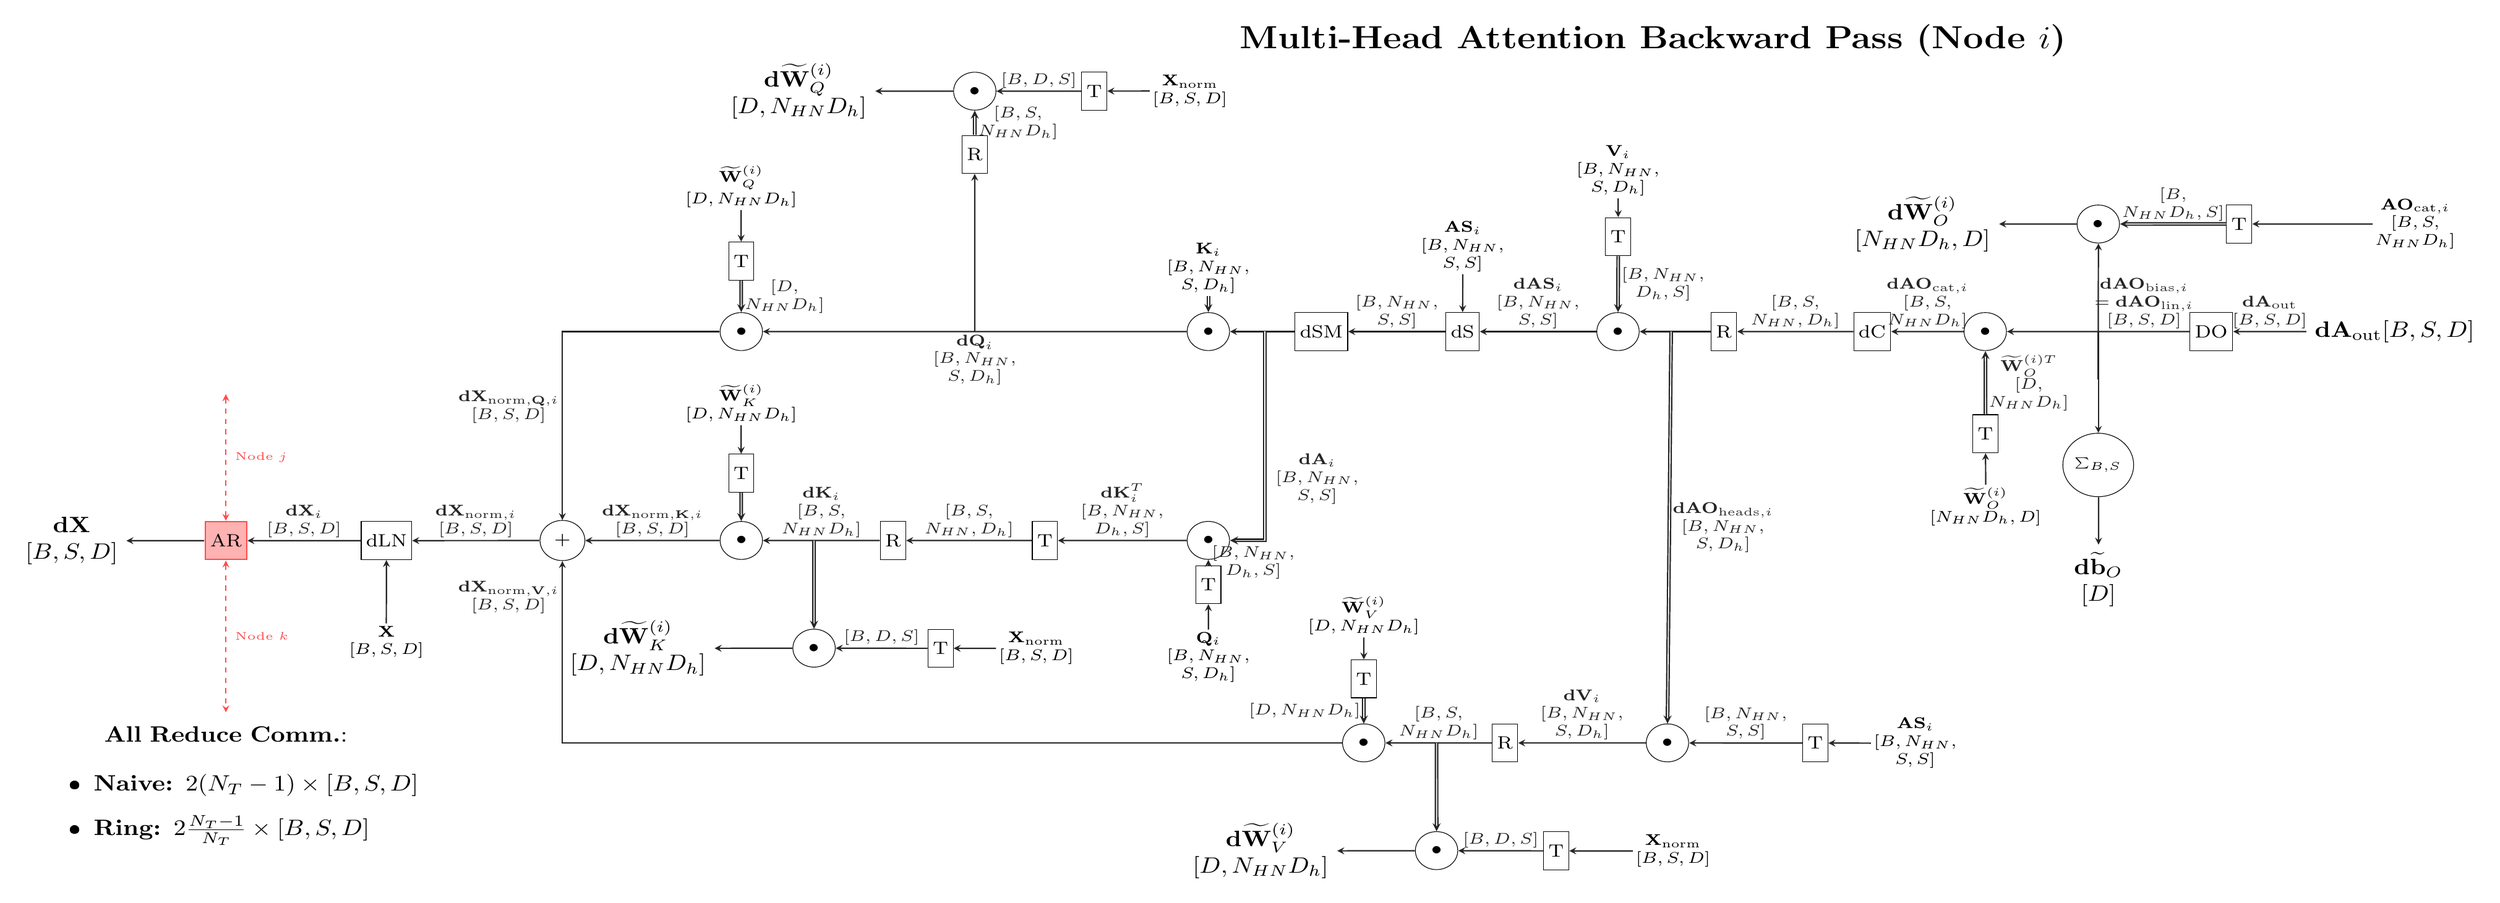
\begin{tikzpicture}[
  every node/.style={transform shape},
  >=stealth,
  auxnode/.style={draw, rectangle, fill=white, minimum height=6mm, inner sep=2pt, font=\footnotesize, align=center},
  mulnode/.style={draw, circle, fill=white, minimum size=6mm, font=\footnotesize, align=center},
  addnode/.style={draw, circle, fill=white, minimum size=6mm, font=\footnotesize, align=center},
  sumnode/.style={draw, circle, fill=white, minimum size=6mm, font=\tiny, align=center},
  allreduce/.style={draw, rectangle, fill=red!30, minimum height=6mm, inner sep=2pt, font=\footnotesize, align=center, thick, draw=red!70},
  flow/.style={->, thick, black!85},
  flow2/.style={->, double, thick, black!85},
  commflow/.style={<->, thick, red!70, dashed},
  dimlabel/.style={font=\scriptsize, inner sep=1pt, align=center},
  gradflow/.style={->, thick, black!85},
  gradweight/.style={->, thick, black!85}
]

\begin{scope}[xscale=1.45, yscale=1.3]

\def\yoffset{-1.0}
\def\dVXyoffset{-6.5}

\coordinate (Grad_Aout_B) at (17.5, \yoffset);
\coordinate (dDrop_center) at (15.9, \yoffset);
\coordinate (ProjGradSplit) at (14.3, \yoffset);
\coordinate (dOProj_center) at (12.7, \yoffset);
\coordinate (C_center) at (11.1, \yoffset);
\coordinate (R_center) at (9.0, \yoffset);
\coordinate (dPV_AS_calc_center) at (7.5, \yoffset);
\coordinate (dSoft_center) at (5.3, \yoffset);
\coordinate (dSM_calc_center) at (3.3, \yoffset);
\coordinate (dV_calc_center) at (8.2, \dVXyoffset+\yoffset);
\coordinate (R_V_bwd_center) at (5.9, \dVXyoffset+\yoffset);
\coordinate (dVX_calc_center) at (3.9, \dVXyoffset+\yoffset);
\coordinate (dQK_calc_Q_center) at (1.7, \yoffset);
\coordinate (dQK_calc_K_center) at (1.7, -3.3+\yoffset);
\coordinate (K_BWD_input_center) at (1.7, 1.0+\yoffset);
\coordinate (T_Q_bwd_center) at (1.7, -4.0+\yoffset);

\node[font=\Large\bfseries] at (8, 4.6+\yoffset) {Multi-Head Attention Backward Pass (Node $i$)};

\node (Grad_Aout_B) at (18.5, \yoffset) {$\mathbf{dA}_{\text{out}}$\\$[B,S,D]$};
\node[auxnode] (DO) at (dDrop_center) {DO};
\node[mulnode] (dOProj) at (dOProj_center) {$\bullet$};

\node[auxnode] (T_WO) [below=1.0cm of dOProj] {T};
\node[dimlabel] (WO_BWD) [below=0.5cm of T_WO] {$\widetilde{\mathbf{W}}_{O}^{(i)}$\\$[N_{HN}D_h,D]$};

\node[mulnode] (dWO_calc) at ($(ProjGradSplit)+(0, 1.7)$) {$\bullet$};
\node[align=center, left=1.1cm of dWO_calc]
  (dWO_GRAD) {$\mathbf{d}\widetilde{\mathbf{W}}_{O}^{(i)}$\\$[N_{HN}D_h,D]$};
\node[auxnode] (T_AO_in) [right=1.5cm of dWO_calc] {T};
\node[dimlabel] (AO_in_local_label) [right=1.7cm of T_AO_in] {$\mathbf{AO}_{\text{cat},i}$\\$[B,S,$\\$N_{HN}D_h]$};

\node[auxnode] (C) at (C_center) {dC};
\node[auxnode] (R) at (R_center) {R};

\node[mulnode] (dPV_AS_calc) at (dPV_AS_calc_center) {$\bullet$};
\node[auxnode] (dSoft) at (dSoft_center) {dS};
\node[auxnode] (dSM_calc) at (dSM_calc_center) {dSM};

\node[mulnode] (dQK_calc_Q) at (dQK_calc_Q_center) {$\bullet$};
\node[mulnode] (dQX_proj_calc) [left=6.0cm of dQK_calc_Q] {$\bullet$};

\node[mulnode] (dQK_calc_K) at (dQK_calc_K_center) {$\bullet$};
\node[mulnode] (dKX_proj_calc) [left=6.0cm of dQK_calc_K] {$\bullet$};

\node[dimlabel] (K_BWD_input) at (K_BWD_input_center) {$\mathbf{K}_i$\\$[B,N_{HN},$\\$S,D_h]$};
\node[auxnode] (T_Q_bwd) at (T_Q_bwd_center) {T};
\node[dimlabel] (Q_BWD_input) [below=0.4cm of T_Q_bwd] {$\mathbf{Q}_i$\\$[B,N_{HN},$\\$S,D_h]$};

\node[dimlabel] (V_FWD) [above=1.8cm of dPV_AS_calc] {$\mathbf{V}_i$\\$[B,N_{HN},$\\$S,D_h]$};
\node[auxnode] (T_V_bwd) [below=0.3cm of V_FWD] {T};

\node[mulnode] (dV_calc) at (dV_calc_center) {$\bullet$};
\node[auxnode] (T_AS_bwd) [right=1.6cm of dV_calc] {T};
\node[dimlabel] (AS_BWD_for_V) [right=0.6cm of T_AS_bwd] {$\mathbf{AS}_i$\\$[B,N_{HN},$\\$S,S]$};

\node[auxnode] (R_V_bwd) at (R_V_bwd_center) {R};
\node[mulnode] (dVX_calc) at (dVX_calc_center) {$\bullet$};

\node[auxnode] (T_WV) [above=0.4cm of dVX_calc] {T};
\node[dimlabel] (WV_BWD) [above=0.35cm of T_WV] {$\widetilde{\mathbf{W}}_{V}^{(i)}$\\$[D,N_{HN}D_h]$};

\node[sumnode] (Sum_dBO) [below=1.6cm of ProjGradSplit] {$\sum_{B, S}$};
\node (dBO) [align=center, below=0.75cm of Sum_dBO] {$\mathbf{d}\widetilde{\mathbf{b}}_{O}$\\$[D]$};

\draw[gradflow] (Grad_Aout_B) -- (DO)
  node[dimlabel, midway, above]{$\mathbf{dA}_{\text{out}}$\\$[B,S,D]$};

\draw[gradflow] (DO) -- (dOProj)
  node[dimlabel, pos=0.25, above]{$\mathbf{dAO}_{\text{bias},i}$\\$=\mathbf{dAO}_{\text{lin},i}$\\$[B,S,D]$};

\draw[gradflow] (ProjGradSplit) -- (dWO_calc.south);
\draw[gradflow] (ProjGradSplit) -- ([yshift=-0.75cm]ProjGradSplit) -| (Sum_dBO.north);

\draw[gradflow] (dOProj) -- (C)
  node[dimlabel, midway, above]{$\mathbf{dAO}_{\text{cat},i}$\\$[B,S,$\\$N_{HN}D_h]$};
\draw[gradflow] (C) -- (R)
  node[dimlabel, midway, above]{$[B,S,$\\$N_{HN},D_h]$};

\coordinate (R_split_point) at ($(dPV_AS_calc)!0.5!(R)$);
\draw[gradflow] (R.west) -- (dPV_AS_calc.east);
\draw[flow2] (R_split_point) -- (dV_calc.north)
  node[dimlabel, midway, right]{$\mathbf{dAO}_{\text{heads},i}$\\$[B,N_{HN},$\\$S,D_h]$};

\draw[gradflow] (V_FWD.south) -- (T_V_bwd.north);
\draw[flow2] (T_V_bwd.south) -- (dPV_AS_calc.north)
  node[dimlabel, midway, right]{$[B,N_{HN},$\\$D_h,S]$};
\draw[gradflow] (dPV_AS_calc.west) -- (dSoft.east)
  node[dimlabel, midway, above]{$\mathbf{dAS}_i$\\$[B,N_{HN},$\\$S,S]$};

\node (AS_BWD_dS) [dimlabel, above=0.6cm of dSoft] {$\mathbf{AS}_i$\\$[B,N_{HN},$\\$S,S]$};
\draw[gradflow] (AS_BWD_dS.south) -- (dSoft.north);
\draw[gradflow] (dSoft.west) -- (dSM_calc.east)
  node[dimlabel, midway, above]{$[B,N_{HN},$\\$S,S]$};

\coordinate (dA_Split_X) at ($(dSM_calc_center)!0.5!(dQK_calc_Q_center)$);
\coordinate (dA_Split) at (dA_Split_X |- dQK_calc_Q.east);
\draw[gradflow] (dSM_calc.west) -- (dQK_calc_Q.east);
\draw[flow2] (dA_Split) -- (dA_Split |- dQK_calc_K.east) -- (dQK_calc_K.east)
  node[dimlabel, pos=-1.5, above, yshift=15]{$\mathbf{dA}_i$\\$[B,N_{HN},$\\$S,S]$};

\draw[flow2] (K_BWD_input.south) -- (dQK_calc_Q.north);
\draw[gradweight] (dQK_calc_Q) -- (dQX_proj_calc)
  node[dimlabel, midway, below]{$\mathbf{dQ}_i$\\$[B,N_{HN},$\\$S,D_h]$};

\node[auxnode] (T_WQ_bwd) [above=0.5cm of dQX_proj_calc] {T};
\node[dimlabel] (WQ_bwd) [above=0.5cm of T_WQ_bwd] {$\widetilde{\mathbf{W}}_{Q}^{(i)}$\\$[D,N_{HN}D_h]$};
\draw[flow] (WQ_bwd) -- (T_WQ_bwd);
\draw[flow2] (T_WQ_bwd.south) -- (dQX_proj_calc.north)
  node[dimlabel, midway, right]{$[D,$\\$N_{HN}D_h]$};

\draw[flow] (Q_BWD_input.north) -- (T_Q_bwd.south);
\draw[flow] (T_Q_bwd.north) -- (dQK_calc_K.south)
  node[dimlabel, pos=0.55, right]{$[B,N_{HN},$\\$D_h,S]$};

\node[auxnode] (T_dK) at ($(dQK_calc_K)!0.35!(dKX_proj_calc)$) {T};
\node[auxnode] (R_dK_mid) at ($(T_dK)!0.5!(dKX_proj_calc)$) {R};

\draw[gradweight] (dQK_calc_K) -- (T_dK)
  node[dimlabel, midway, above]{$\mathbf{dK}_i^T$\\$[B,N_{HN},$\\$D_h,S]$};
\draw[gradweight] (T_dK) -- (R_dK_mid)
  node[dimlabel, midway, above]{$[B,S,$\\$N_{HN},D_h]$};
\draw[gradweight] (R_dK_mid) -- (dKX_proj_calc)
  node[dimlabel, midway, above]{$\mathbf{dK}_i$\\$[B,S,$\\$N_{HN}D_h]$};

\node[auxnode] (T_WK_bwd) [above=0.45cm of dKX_proj_calc] {T};
\node[dimlabel] (WK_bwd) [above=0.45cm of T_WK_bwd] {$\widetilde{\mathbf{W}}_{K}^{(i)}$\\$[D,N_{HN}D_h]$};
\draw[gradflow] (WK_bwd) -- (T_WK_bwd);
\draw[flow2] (T_WK_bwd.south) -- (dKX_proj_calc.north);

\draw[gradflow] (AS_BWD_for_V.west) -- (T_AS_bwd.east);
\draw[gradflow] (T_AS_bwd.west) -- (dV_calc.east)
  node[dimlabel, midway, above]{$[B,N_{HN},$\\$S,S]$};
\draw[gradflow] (dV_calc.west) -- (R_V_bwd.east)
  node[dimlabel, midway, above]{$\mathbf{dV}_i$\\$[B,N_{HN},$\\$S,D_h]$};
\draw[gradflow] (R_V_bwd) -- (dVX_calc.east)
  node[dimlabel, midway, above]{$[B,S,$\\$N_{HN}D_h]$};

\draw[gradflow] (WV_BWD) -- (T_WV);
\draw[flow2] (T_WV) -- (dVX_calc.north)
  node[dimlabel, midway, left]{$[D,N_{HN}D_h]$};

\node[addnode] (Sum_dXnorm) [left=1.9cm of dKX_proj_calc] {$+$};

\draw[gradweight] (dQX_proj_calc.west) -| node[dimlabel, pos=0.7, left]{$\mathbf{dX}_{\text{norm},\mathbf{Q},i}$\\$[B,S,D]$} (Sum_dXnorm.north);
\draw[gradweight] (dKX_proj_calc.west) -- node[dimlabel, midway, above]{$\mathbf{dX}_{\text{norm},\mathbf{K},i}$\\$[B,S,D]$} (Sum_dXnorm.east);
\draw[gradweight] (dVX_calc.west) -| node[dimlabel, pos=0.9, left]{$\mathbf{dX}_{\text{norm},\mathbf{V},i}$\\$[B,S,D]$} (Sum_dXnorm.south);

\coordinate (dV_branch) at ($(R_V_bwd.west)!0.52!(dVX_calc.east)$);
\node[mulnode] (dWV_mul) at ($(dV_branch)+(0,-1.7cm)$) {$\bullet$};
\draw[flow2] (dV_branch) -- (dWV_mul.north);

\node[auxnode] (T_Xnorm) [right=1.2cm of dWV_mul] {T};
\node[dimlabel] (Xnorm_local) [right=0.9cm of T_Xnorm] {$\mathbf{X}_{\text{norm}}$\\$[B,S,D]$};
\draw[gradflow] (Xnorm_local) -- (T_Xnorm);
\draw[gradflow] (T_Xnorm.west) -- (dWV_mul.east)
  node[dimlabel, midway, above]{$[B,D,S]$};
\node (dWV_out) [align=center, left=1.1cm of dWV_mul] {$\mathbf{d}\widetilde{\mathbf{W}}_{V}^{(i)}$\\$[D,N_{HN}D_h]$};
\draw[gradweight] (dWV_mul.west) -- (dWV_out);

\coordinate (dQ_branch) at ($(dQK_calc_Q.east)!0.50!(dQX_proj_calc.west)$);
\node[mulnode] (dWQ_mul) at ($(dQ_branch)+(0,3.8cm)$) {$\bullet$};
\node[auxnode] (R_dQ_for_WQ) at ($(dWQ_mul)+(0,-1.0cm)$) {R};
\draw[gradflow]  (dQ_branch) -- (R_dQ_for_WQ.south);
\draw[flow2] (R_dQ_for_WQ.north) -- (dWQ_mul.south)
  node[dimlabel, midway, right]{$[B,S,$\\$N_{HN}D_h]$};

\node[auxnode] (T_XnormQ) [right=1.2cm of dWQ_mul] {T};
\node[dimlabel] (Xnorm_localQ) [right=0.6cm of T_XnormQ] {$\mathbf{X}_{\text{norm}}$\\$[B,S,D]$};
\draw[gradflow] (Xnorm_localQ) -- (T_XnormQ);
\draw[gradflow] (T_XnormQ.west) -- (dWQ_mul.east)
  node[dimlabel, midway, above]{$[B,D,S]$};
\node (dWQ_out) [align=center, left=1.1cm of dWQ_mul] {$\mathbf{d}\widetilde{\mathbf{W}}_{Q}^{(i)}$\\$[D,N_{HN}D_h]$};
\draw[gradweight] (dWQ_mul.west) -- (dWQ_out);

\coordinate (dK_branch) at ($(R_dK_mid)!0.52!(dKX_proj_calc)$);
\node[mulnode] (dWK_mul) at ($(dK_branch)+(0,-1.7cm)$) {$\bullet$};
\draw[flow2]  (dK_branch) -- (dWK_mul.north);

\node[auxnode] (T_XnormK) [right=1.3cm of dWK_mul] {T};
\node[dimlabel, right=0.6cm of T_XnormK] (Xnorm_localK) {$\mathbf{X}_{\text{norm}}$\\$[B,S,D]$};
\draw[gradflow] (Xnorm_localK) -- (T_XnormK);
\draw[gradflow] (T_XnormK.west) -- (dWK_mul.east)
  node[dimlabel, midway, above]{$[B,D,S]$};
\node (dWK_out) [align=center, left=1.1cm of dWK_mul] {$\mathbf{d}\widetilde{\mathbf{W}}_{K}^{(i)}$\\$[D,N_{HN}D_h]$};
\draw[gradweight] (dWK_mul.west) -- (dWK_out);

\draw[gradweight] (Sum_dBO) -- (dBO);

\draw[gradflow] (WO_BWD) -- (T_WO);
\draw[flow2] (T_WO) -- (dOProj)
  node[dimlabel, midway, right]{$\widetilde{\mathbf{W}}_{O}^{(i)T}$\\$[D,$\\$N_{HN}D_h]$};
\draw[gradflow] (AO_in_local_label) -- (T_AO_in);
\draw[flow2] (T_AO_in) -- (dWO_calc.east)
  node[dimlabel, midway, above]{$[B,$\\$N_{HN}D_h,S]$};
\draw[gradweight] (dWO_calc) -- (dWO_GRAD);

\node[auxnode] (dLN) [left=1.8cm of Sum_dXnorm] {dLN};
\draw[gradweight] (Sum_dXnorm.west) -- node[dimlabel, midway, above]
  {$\mathbf{dX}_{\text{norm},i}$\\$[B,S,D]$} (dLN.east);

\node[allreduce] (AR) [left=1.6cm of dLN] {AR};
\node[
  align=center,
  below=2.5cm of AR,
  text width=5.5cm
] (AR_info) {%
  \textbf{All Reduce Comm.}:\\[2pt]
  \begin{itemize}
    \item \textbf{Naive:} $2(N_T-1) \times [B,S,D]$
    \item \textbf{Ring:} $2\frac{N_T-1}{N_T} \times [B,S,D]$
  \end{itemize}
};

% All-Reduce communication arrows
\draw[commflow] (AR.north) -- ++(0, 2.0) node[midway, right, font=\tiny]{Node $j$};
\draw[commflow] (AR.south) -- ++(0, -2.4) node[midway, right, font=\tiny]{Node $k$};

\draw[gradweight] (dLN.west) -- (AR.east) node[dimlabel, midway, above]{$\mathbf{dX}_i$\\$[B,S,D]$};

\node (dX_OUT) [align=center, left=1.1cm of AR] {$\mathbf{dX}$\\$[B,S,D]$};
\draw[gradweight] (AR.west) -- (dX_OUT);

\node[dimlabel] (LNCache) [below=1.0cm of dLN] {$\mathbf{X}$\\$[B,S,D]$};
\draw[gradflow] (LNCache.north) -- (dLN.south);

\end{scope}
\end{tikzpicture}
}

\subsection{Communication Patterns}
\textit{[To be added]}

\clearpage

\section{Data Parallelism (DP)}
\subsection{DP Overview}

    \resizebox{\linewidth}{!}{%
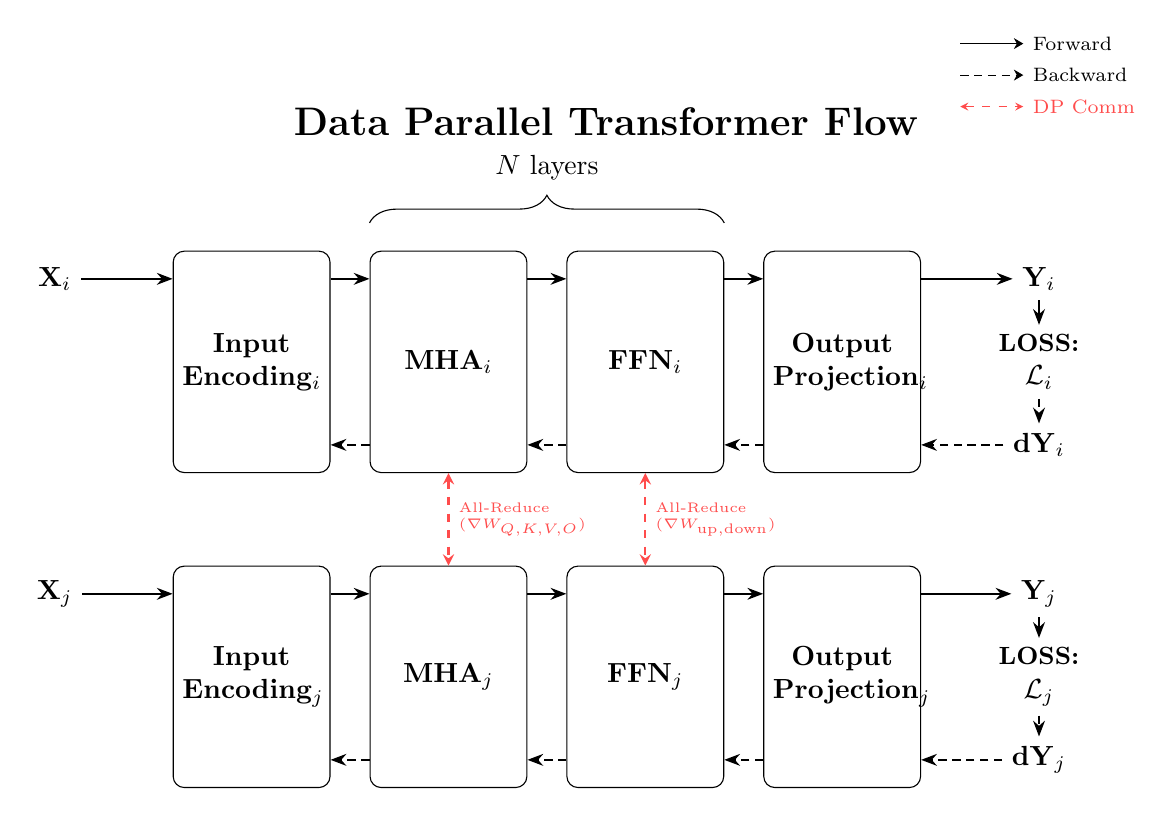
\begin{tikzpicture}[
    node distance=2.5cm,
    >=stealth,
    block/.style={rectangle, draw=black, fill=white, text width=5em, text centered, rounded corners, minimum height=8em, font=\bfseries},
    forward/.style={-{Stealth[length=2mm]}, thick, black},
    backward/.style={-{Stealth[length=2mm]}, thick, black, densely dashed},
    dpcomm/.style={<->, thick, red!70, dashed},
    io/.style={text centered, font=\bfseries}
]
    % Title
    \node[font=\Large\bfseries] at (7, 12) {Data Parallel Transformer Flow};

    % ========== Node i (Upper) ==========
    \node (input_i) [io] at (0, 10) {$\mathbf{X}_i$};
    \node (encoding_i) [block, right of=input_i, yshift=-3em] {Input\\Encoding$_i$};
    \node (mha_i) [block, right of=encoding_i] {MHA$_i$};
    \node (mlp_i) [block, right of=mha_i] {FFN$_i$};
    \node (output_i) [block, right of=mlp_i] {Output\\Projection$_i$};
    \node (pred_i) [io, right of=output_i, yshift=3em] {$\mathbf{Y}_i$};
    \node (loss_i) [align=center, io, right of=output_i] {\small LOSS:\\$\mathcal{L}_i$};
    \node (gradient_i) [io, right of=output_i, yshift=-3em] {$\mathbf{dY}_i$};

    % Forward arrows - Node i
    \draw [forward] (input_i) -- ([yshift=3em]encoding_i.west);
    \draw [forward] ([yshift=3em]encoding_i.east) -- ([yshift=3em]mha_i.west);
    \draw [forward] ([yshift=3em]mha_i.east) -- ([yshift=3em]mlp_i.west);
    \draw [forward] ([yshift=3em]mlp_i.east) -- ([yshift=3em]output_i.west);
    \draw [forward] ([yshift=3em]output_i.east) -- (pred_i);
    \draw [forward] (pred_i) -- (loss_i);
    \draw [backward] (loss_i) -- (gradient_i);

    % Backward arrows - Node i
    \draw [backward] (gradient_i) -- ([yshift=-3em]output_i.east);
    \draw [backward] ([yshift=-3em]output_i.west) -- ([yshift=-3em]mlp_i.east);
    \draw [backward] ([yshift=-3em]mlp_i.west) -- ([yshift=-3em]mha_i.east);
    \draw [backward] ([yshift=-3em]mha_i.west) -- ([yshift=-3em]encoding_i.east);

    % Brace for layer repetition - Node i
    \draw[decorate, decoration={brace, amplitude=10pt}]
        ([yshift=1.0em]mha_i.north west) -- ([yshift=1.0em]mlp_i.north east)
        node[midway, above=12pt, font=\normalsize] {$N$ layers};

    % ========== Node j (Lower) ==========
    \node (input_j) [io] at (0, 6) {$\mathbf{X}_j$};
    \node (encoding_j) [block, right of=input_j, yshift=-3em] {Input\\Encoding$_j$};
    \node (mha_j) [block, right of=encoding_j] {MHA$_j$};
    \node (mlp_j) [block, right of=mha_j] {FFN$_j$};
    \node (output_j) [block, right of=mlp_j] {Output\\Projection$_j$};
    \node (pred_j) [io, right of=output_j, yshift=3em] {$\mathbf{Y}_j$};
    \node (loss_j) [align=center, io, right of=output_j] {\small LOSS:\\$\mathcal{L}_j$};
    \node (gradient_j) [io, right of=output_j, yshift=-3em] {$\mathbf{dY}_j$};

    % Forward arrows - Node j
    \draw [forward] (input_j) -- ([yshift=3em]encoding_j.west);
    \draw [forward] ([yshift=3em]encoding_j.east) -- ([yshift=3em]mha_j.west);
    \draw [forward] ([yshift=3em]mha_j.east) -- ([yshift=3em]mlp_j.west);
    \draw [forward] ([yshift=3em]mlp_j.east) -- ([yshift=3em]output_j.west);
    \draw [forward] ([yshift=3em]output_j.east) -- (pred_j);
    \draw [forward] (pred_j) -- (loss_j);
    \draw [backward] (loss_j) -- (gradient_j);

    % Backward arrows - Node j
    \draw [backward] (gradient_j) -- ([yshift=-3em]output_j.east);
    \draw [backward] ([yshift=-3em]output_j.west) -- ([yshift=-3em]mlp_j.east);
    \draw [backward] ([yshift=-3em]mlp_j.west) -- ([yshift=-3em]mha_j.east);
    \draw [backward] ([yshift=-3em]mha_j.west) -- ([yshift=-3em]encoding_j.east);

    % ========== DP Communications ==========
    \draw [dpcomm] (mha_i.south) -- (mha_j.north) node[midway, right, font=\tiny, align=left] {All-Reduce\\$(\nabla W_{Q,K,V,O})$};
    \draw [dpcomm] (mlp_i.south) -- (mlp_j.north) node[midway, right, font=\tiny, align=left] {All-Reduce\\$(\nabla W_{\text{up},\text{down}})$};

    % Labels (Legend)
    \coordinate (legend) at ([xshift=11.5cm, yshift=8.5em]input_i);

    % Forward (작은 화살표 + 작은 글자)
    \draw[
        forward,
        -{Stealth[length=1.2mm,width=1.4mm]}, % 화살표 더 작게
        line width=0.3pt                       % 선 더 얇게
    ] (legend) -- ++(0.8,0)
      node[right, font=\scriptsize] {Forward};

    % Backward
    \draw[
        backward,
        -{Stealth[length=1.2mm,width=1.4mm]},
        line width=0.3pt
    ] ([yshift=-0.4cm]legend) -- ++(0.8,0)
      node[right, font=\scriptsize] {Backward};

    % DP Comm
    \draw[
        dpcomm,
        line width=0.3pt
    ] ([yshift=-0.8cm]legend) -- ++(0.8,0)
      node[right, font=\scriptsize] {DP Comm};
\end{tikzpicture}%
}


\end{document}